%
% Unless otherwise indicated, the copyright in this material is 
% owned by Joerg Evermann. This material is licensed to you under the 
% Creative Commons by-attribution non-commercial license (CC BY-NC 4.0)}
%

\section*{Sources and Further Reading}

The material in this chapter is based on the following sources. 

\begin{tcolorbox}[colback=alert]
Treveil, M. and the Dataiku Team (2020) \emph{Introducing MLOps}, O'Reilly Media, Sebastopol, CA (T) 
\end{tcolorbox}

The book by Mark Treveil and others is a good, short introduction to the principles and ideas of machine learning operations. It provides guidance on the process, the management, and the governance of MLOps. Given its focus on high-level introduction, it provides few technical details, but this also means that this book will likely stay relevant longer. 


\begin{tcolorbox}[colback=alert]
Gift, N. and Deza, Al. (2021) \emph{Practical MLOps}, O'Reilly Media, Sebastopol, CA (GD)
\end{tcolorbox}

The book by Noah Gift and Alfredo Deza provides a more ''hands-on'' introduction to machine learning operations. While also touching on the principles and processes, it goes in-depth and offers specific technical illustrations of good MLOps practices. The book uses both on-premises technology and cloud-based technologies, but focuses most heavily on MLOps on the AWS cloud. 


\begin{tcolorbox}[colback=alert]
\subsubsection*{Resources}
Complete implementations of all examples in this chapter are available on the following GitHub repo:

\url{https://github.com/jevermann/busi4720-mlops} \\

The project can be cloned from this URL:

\url{https://github.com/jevermann/busi4720-mlops.git}
\end{tcolorbox}


\section{Introduction}

Many introductions to machine learning and predictive models in particular focus on the different types of statistical models, their properties and relative advantages, and challenges and best-practices for feature engineering and model training. Using the R or Python environment, the focus is often on the business analytics team that identifies features and creates the model. A frequent implicit assumption is that this happens in isolation, on relatively small data sets, and on desktop computers. Often, such an introduction fails to examine not only infrastructure challenges but, more importantly, also neglects to examine how the created models are managed and used productively. The latter is arguably most important from a business perspective.

As an example, consider a dynamic pricing model that predicts what customers are willing to spend on a particular product based on their previous purchase history and other features. It is relatively easy to collect a small data set and train a few different models. However, ultimately, this model must be integrated with the web-based store front of the organization and will be used to show different prices to different customers. It is a long way from a small model on the desktop to a model that is in production use within an organization's larger set of software applications. Besides problems of efficiently moving models to production, that is, ''\emph{deploying}'' them, models in production also pose certain risks to an organization and these risks must be managed. 

\subsection*{Purpose}

Machine Learning Operations, or MLOps, therefore has three main purposes. First, it seeks to improve operational efficiency in model management and deployment. It does this through formalized and automated processes to achieve reliability and repeatability in deployment. 

The second purpose is to manage and mitigate risk. Different types of risks arise, such as availability of service. What happens when the dynamic pricing model in the example becomes unavailable due to a computer outage or a software misconfiguration? Will the organization lose money? Will it lose customers? Another risk stems from the model quality and the impacts of model predictions. For example, how large are the prediction errors of the dynamic pricing model and how much potential revenue could the organization lose by overpricing items and causing the customers not to purchase something? How much potential revenue remains unrealized because items are offered at a lower price than a customer would be willing to pay? A third type of risk arises from prediction fairness. For example if the pricing model includes features such as gender so that different prices are offered to men and women, would that be fair (or even legally allowed)? If this were to become widely known to customers, would customers defect from the business? Finally, there is the risk of skill loss. What happens when the business analysts who developed the model leave the organization? Does the organization have sufficient documentation for auditability and risk management? Can the model be recreated by a new team? How easily can a replacement team member become familiar with a model and its history, rationale, and current uses?

The third purpose of MLOps is to establish accountability, auditability, and traceability. Accountability is concerned with decisions made about models, their acceptance, and their deployment into production. It requires formalized testing and acceptance procedures for the model as it moves from data extraction to deployment. This begins with questions whether there is legal or ethical clearance to use a particular data set, to the decision as to when a new model replaces an existing model in a production environment, e.g. in the web-based store front of the dynamic pricing example. Auditability and traceability have two aspects. First, they refer to internal processes and procedures and concern the ability to answer questions about the origins of the training data, of the model parameters, the production environment, and related decisions, for example about feature inclusion or risk assessment. A second aspect is the auditability and traceability of model output and/or decisions made based on the model output. In the dynamic pricing model example, the organization must maintain a record of why a certain price was offered to a particular customer, what the relevant features were that led to the decision, and be able to trace these features back through the model all the way to the training data. 

\subsection*{Challenges}

As business analytics, machine learning, and predictive models have become popular, organizations face a number of challenges. First, the popularity and the competitive necessity for organizations to engage in this area often leads to a proliferation of separate business analytics teams in different organizational units, that produce a multitude of models, from a wide variety of data, for a large number of potential use cases. In many organizations, machine learning is not well organized and managed, leading to conflicting goals, unanticipated model interactions, lack of traceability and auditability, lack of compliance, lack of knowledge of model performance, lack of accountability and, in the worst case, customer-facing problems where the organization's customers that are affected by a predictive model's decisions become aware of its poor quality. 

A second challenge is the fact that data is constantly changing. After a model has been trained, the organization continues to receive or collect data that can and should be used for model training. If nothing else, additional training data can reduce the prediction error of the model. However, the main challenge is that data may change over time. For example, the business may attract customers with different characteristics and needs, or the industry competitive position of a business may change so that customers have different preferences, or the macro-economic conditions may change to make customers more risk averse or less willing to spend money. These challenges can lead to models that perform poorly, and require a systematic approach to model performance monitoring, model retraining, and tracking the relative performance of different models and different model versions.

As a third challenge, the needs of the business or organization can change over time, making predictive models irrelevant or ill-suited for their purpose. Organizations may shift their strategies, enter or exit specific markets, adapt their marketing strategies and tactics, change their business processes and operations and many other aspects. Such changes will affect the usefulness of predictive models that are deployed in the organization and may require replacing or retraining models, perhaps with new input features, different targets, and with trained with loss functions more appropriate to the changed business goals and objectives. 

A fourth challenge is the mixed composition of business analytics teams. Such teams are often comprised of business professionals as subject matter experts, data scientists that focus on data quality, data provenance, and model development, software engineers that must take a trained model and embed it into an organization's software applications, for example, into their web-based sales tool or their mobile app. Finally, IT staff participate on teams to provision appropriate infrastructure and manage IT related risk. The problem with such interdisciplinary teams is often that people may be unaware of the roles or the importance of others on the team, they may be focused on optimizing their particular aspect of model development to the detriment of the overall effort, they may use different terminology (for example, what precisely does the term ''model'' mean to each of them?), and they may not have developed effective management processes or means of communication. 

Finally, data scientists tend to have little expertise in software engineering and software deployment. Traditionally, this role has focused on the specific details of the statistical models without any reference to established practices that makes software products reliable, robust, scalable, easily maintainable, auditable, fault and failure tolerant, safe, or a variety of other desirable properties. However, when machine learning models or predictive or prescriptive models and algorithms are to be deployed within an organization or even facing an organization's customers, the models become part of an organization's software and therefore such software properties become very important, possibly more important than the predictive accuracy of a machine learning model. 

\subsection*{Principles}

MLOps is a set of practices based on a few main principles. The first principle is that of reliability and reproducibility of operations. This requires standardized and structured processes that are made explicit, either in the form of documentation or, if they are automated, in the form of programming code. Such a process typically includes the steps beginning with data extraction from operational systems, data preprocessing and cleaning, feature extraction and feature engineering, training and evaluation of multiple models, hyper-parameter search, automated model testing, automated software building, and ending with automated deployment. Each process step must be documented and the results archived for auditability purposes. 

It is clear that describing the process with executable code, e.g. in the form of Python scripts or using a variety of open-source or cloud-based products, is preferable to simply writing out a procedure manual. This preference for code illustrates the second main principle of MLOps, that of robust automation. Together, the first two principles ensure that every model in production can be easily re-created in identical form when needed. More importantly, for auditability purposes, the principles ensure that the model and data provenance are captured and documented, that decisions and actions as to which model to move into production are documented, and that the organization knows which models are currently in production and what their properties (e.g. error rate, cost, resource consumption, risk assessment results, etc.) are.

A frequently used term related to robust automation is that of ''infrastructure as code''. Modern development, testing, and production environments are often provisioned automatically. That is, computer servers, software, databases, file storage are provided automatically as needed. To enable this, the requirements for a particular model and how to provide or create them must be described. To take one example, building and deploying a predictive model as a micro-service requires instructions on how to build the software that serves the model predictions (e.g. a Makefile\footnote{A Makefile contains computer readable instructions in a standardized format that allows the ''make'' software tool to automatically build and test a software application. For more details, see this page: \url{https://en.wikipedia.org/wiki/Make_(software)}.}), instructions on how to build the container that the software will run in (e.g. a Dockerfile\footnote{Containers are ''light-weight'' virtual machines with their own operating system, databases, and other software installed in them. Docker is one particular container technology. A Dockerfile defines how to build a docker container, that is, what operating system to use, which software packages to install and how to configure the software in the container for use. For details on containerization see this page: \url{https://en.wikipedia.org/wiki/Containerization_(computing)} and for detail on Docker, see this page: \url{https://en.wikipedia.org/wiki/Docker_(software)}.}), instructions on what type of machine to run the container on, etc. These instructions are themselves computer code and they must be managed, versioned and tested as computer code. 

The third principle is that all versions of both the data and the models must be maintained and managed. Models in this context mean more than just the final parameter values but includes evaluation results, hyper-parameters, training and testing history, model explainability results, model rationale, versions of all software packages that were used, and any other documentation. A variety of open-source and commercial on-premises and cloud-based tools are available for this, ranging from software code versioning tools like git and GitHub to model registries on Amazon Web Services or Microsoft Azure. Versioning of the training data is more problematic, as training data sets can be very large. It is often simply not feasible to keep copies of different versions and more intelligent approaches are being developed. Managing and versioning data and models are useful both for automating model deployment and for ensuring auditability and through this, for ensuring compliance with internal or external requirements. For example, model versioning and management allows an organization to say precisely what features and input data was used to train a model, and what features and their relative importance are being used to make decisions. 

The fourth principle of MLOps is continuous delivery to production. The idea is that rather than treating model development and deployment a single or one-off project, models should be continuously improved and the improved models should be continuously moved into production. That is, as new training data becomes available, model training continues or the existing model can be fine-tuned with the new data. Of course, continuous delivery and integration does not mean to do this whenever a single new training observation becomes available, but to have an established frequency, depending on model size and required training time, of doing continuous delivery daily, weekly, monthly, quarterly or annually. Importantly, training or fine-tuning the model is just the initial step that kicks off the delivery process. Activities like testing, risk assessment, documentation, performance comparison, software integration, etc. need to follow for each newly created model.

Finally, to ensure traceability, auditability, risk management and identify when models should be replaced, retrained or fine-tuned, continuous monitoring of a model in production is required. This means that all inputs and all outputs to the model must be logged and analyzed. In the dynamic pricing model example, this means that whenever a customer is offered a price for an item that is determined by the predictive model, all relevant input features and the model prediction must be logged, as well as the actual purchase decision or other resulting action by the customer. It is obvious that such log data can grow quickly in size and appropriate infrastructure needs to be in place to manage the data. More importantly, procedures and processes need to be in place to actively monitor and analyze this data to detect changes in customer features over time or changes in model accuracy over time. 

\subsection*{Relationship to Other Disciplines}

Machine learning operations (MLOps) is at the intersection of a number of related disciplines, as shown in Figure~\ref{fig:mlopsrelationships}. It overlaps with machine learning where model building, training, evaluation, etc. are located (''ML Model'' in Figure~\ref{fig:mlopsrelationships}. Specifically, MLOps focuses on that part of machine learning that is sometimes called ''CD4ML'' (continuous delivery for machine learning), that is, the software engineering principles of continuous delivery as applied to machine learning models. MLOps overlaps with software engineering, which focuses on continuous integration and continuous delivery (''CI/CD'' in Figure~\ref{fig:mlopsrelationships}, ''DevOps'' (unified or integrated development and operations), and automation of software delivery pipelines. Finally, MLOps overlaps with data engineering, which focuses on collecting, managing, and providing data for organizational purposes, including but not only to machine learning applications. Other uses of data in business analytics may be databases for descriptive analytics or visualizations. 

\begin{figure}
\centering
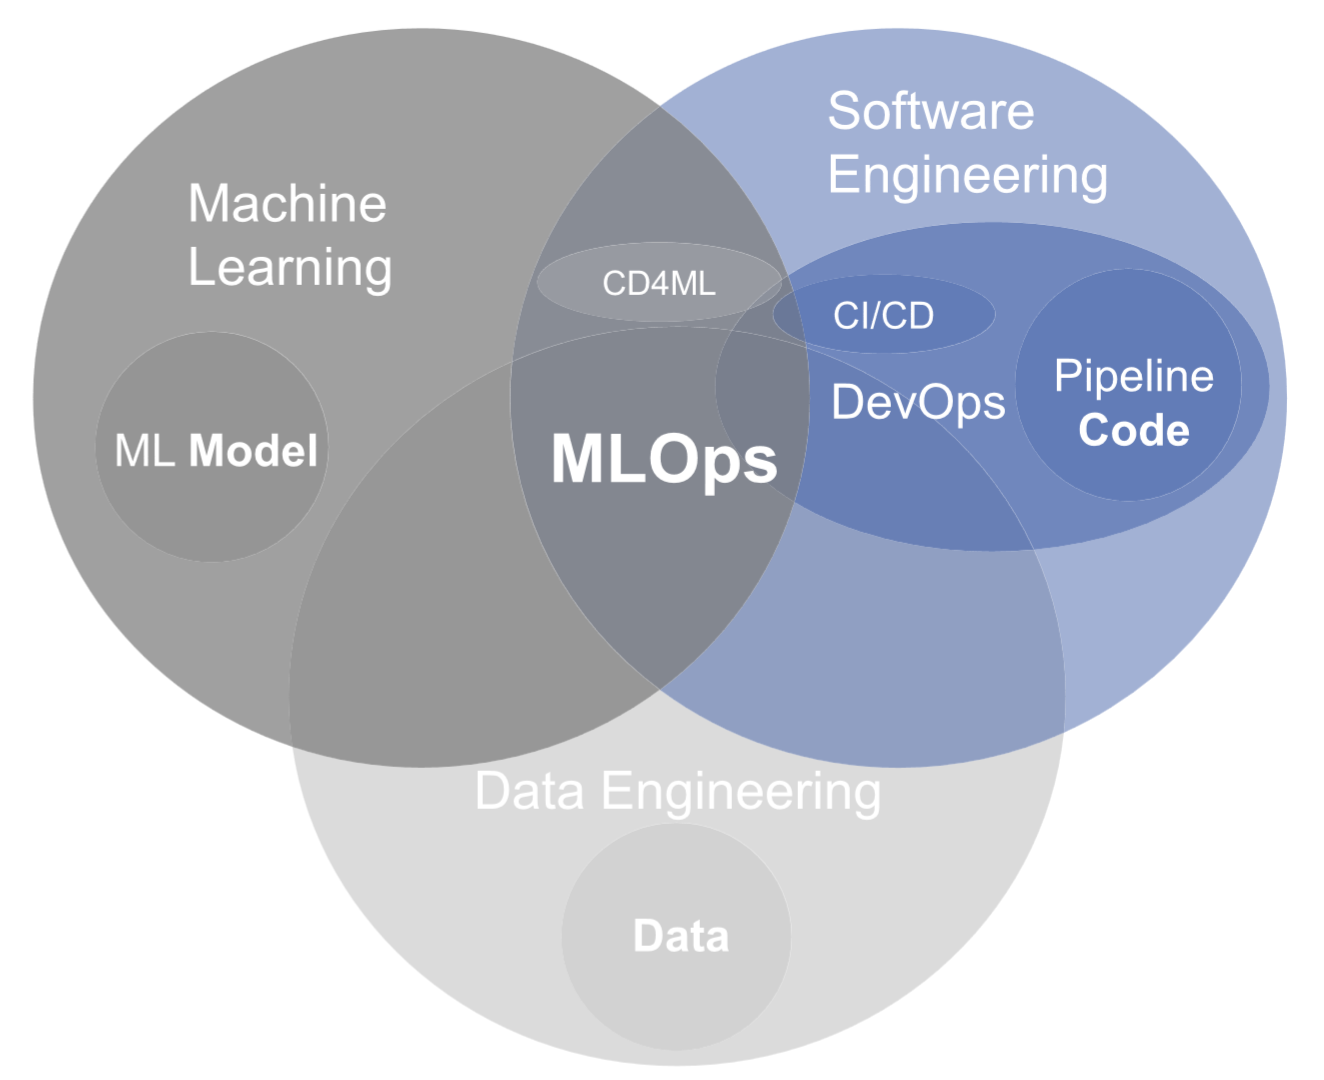
\includegraphics[width=.75\textwidth]{Kreuzbergeretal_fig5.png} \\
\scriptsize \textbf{Source:} \href{https://ieeexplore.ieee.org/abstract/document/10081336}{Kreuzberger, D., K\"uhl, N., \& Hirschl, S. (2023). Machine learning operations (mlops): Overview, definition, and architecture. IEEE access, 11, 31866-31879.}
\caption{MLOps -- Relationship to other disciplines}
\label{fig:mlopsrelationships}
\end{figure}

\section{MLOps Lifecycle Overview}

The MLOps lifecycle is a combination of the machine learning model lifecycle, shown in Figure~\ref{fig:modellifecycle}, and the software development ''DevOps'' lifecycle in Figure~\ref{fig:devopsmodel}. The resulting combination is shown in Figure~\ref{fig:mlopslifecycle}. 

The model development lifecycle in Figure~\ref{fig:modellifecycle} contains activities to manage the data and to develop a machine learning or prediction model. Data collection can include activities such as ETL (''extraction, transformation, loading'') data from source systems, acquisition from external data brokers or vendors, or scraping data from web sites or news sites, or any number of other ways. The data must be curated. For example, its provenance must be established and recorded, it's quality must be assessed, legal or licensing issues must be resolved, etc. The data can then be transformed. This includes both pre-processing for data cleaning as well as engineering new features or combining multiple data sets. Data validation then ensures that the data is of high quality, relevant to the problem, fit for purpose and can legally be used. 

\begin{figure}[h]
\centering
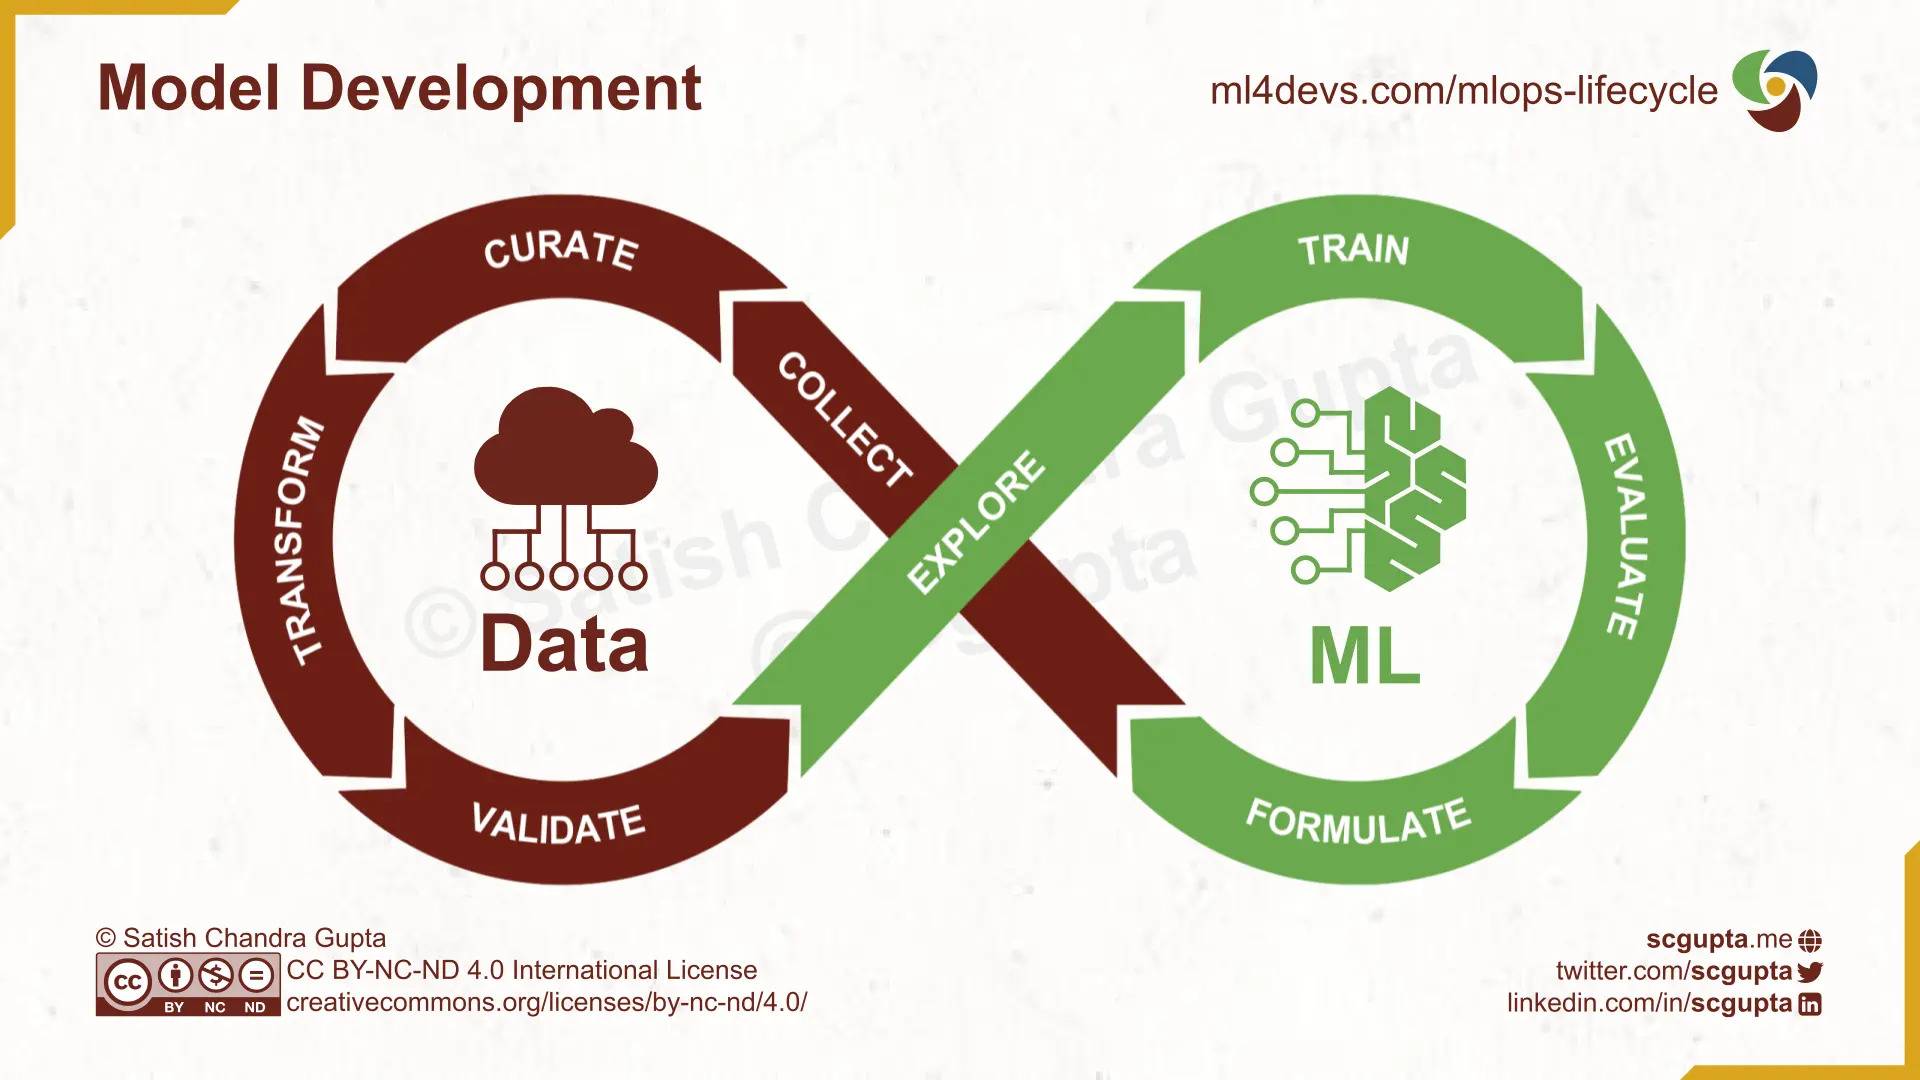
\includegraphics[width=.8\textwidth]{mlmodel.jpeg}
\caption{Model Development Lifecycle}
\label{fig:modellifecycle}
\end{figure}

The model part of the model development lifecycle begins with data exploration, that is, gaining an understanding of the various features, their interactions, summary statistics, etc. This leads to defining and training one or more models on the data set. This step can also include model search (for example, varying the architecture of a neural network model) or hyper-parameter search (for example, finding the optimal depth of a decision tree). The models are then evaluated and compared on suitable metrics, using hold-out samples or cross-validation. Finally, the evaluation results can be used to inform additional data collection or additional features to be used in a better model leading to another iteration of lifecycle.

DevOps (that is, integrated development and operations) is an approach to software development that focuses on continuous integration and continuous deployment. In early software development, a software application was created by developers, typically as a one-off project, and then turned over to the IT operations department to put it into production. Having separate teams for development and operations leads to problems and frictions. For example, the development team might not be concerned with how much resources their application will require or what operational or security risks an application poses. This puts significant pressure on the operations team. The DevOps approach to software development focuses on an integrated process and integrated teams. Rather than developing software in large one-off projects, DevOps encourages continuous improvement. 

\begin{figure}[h]
\centering
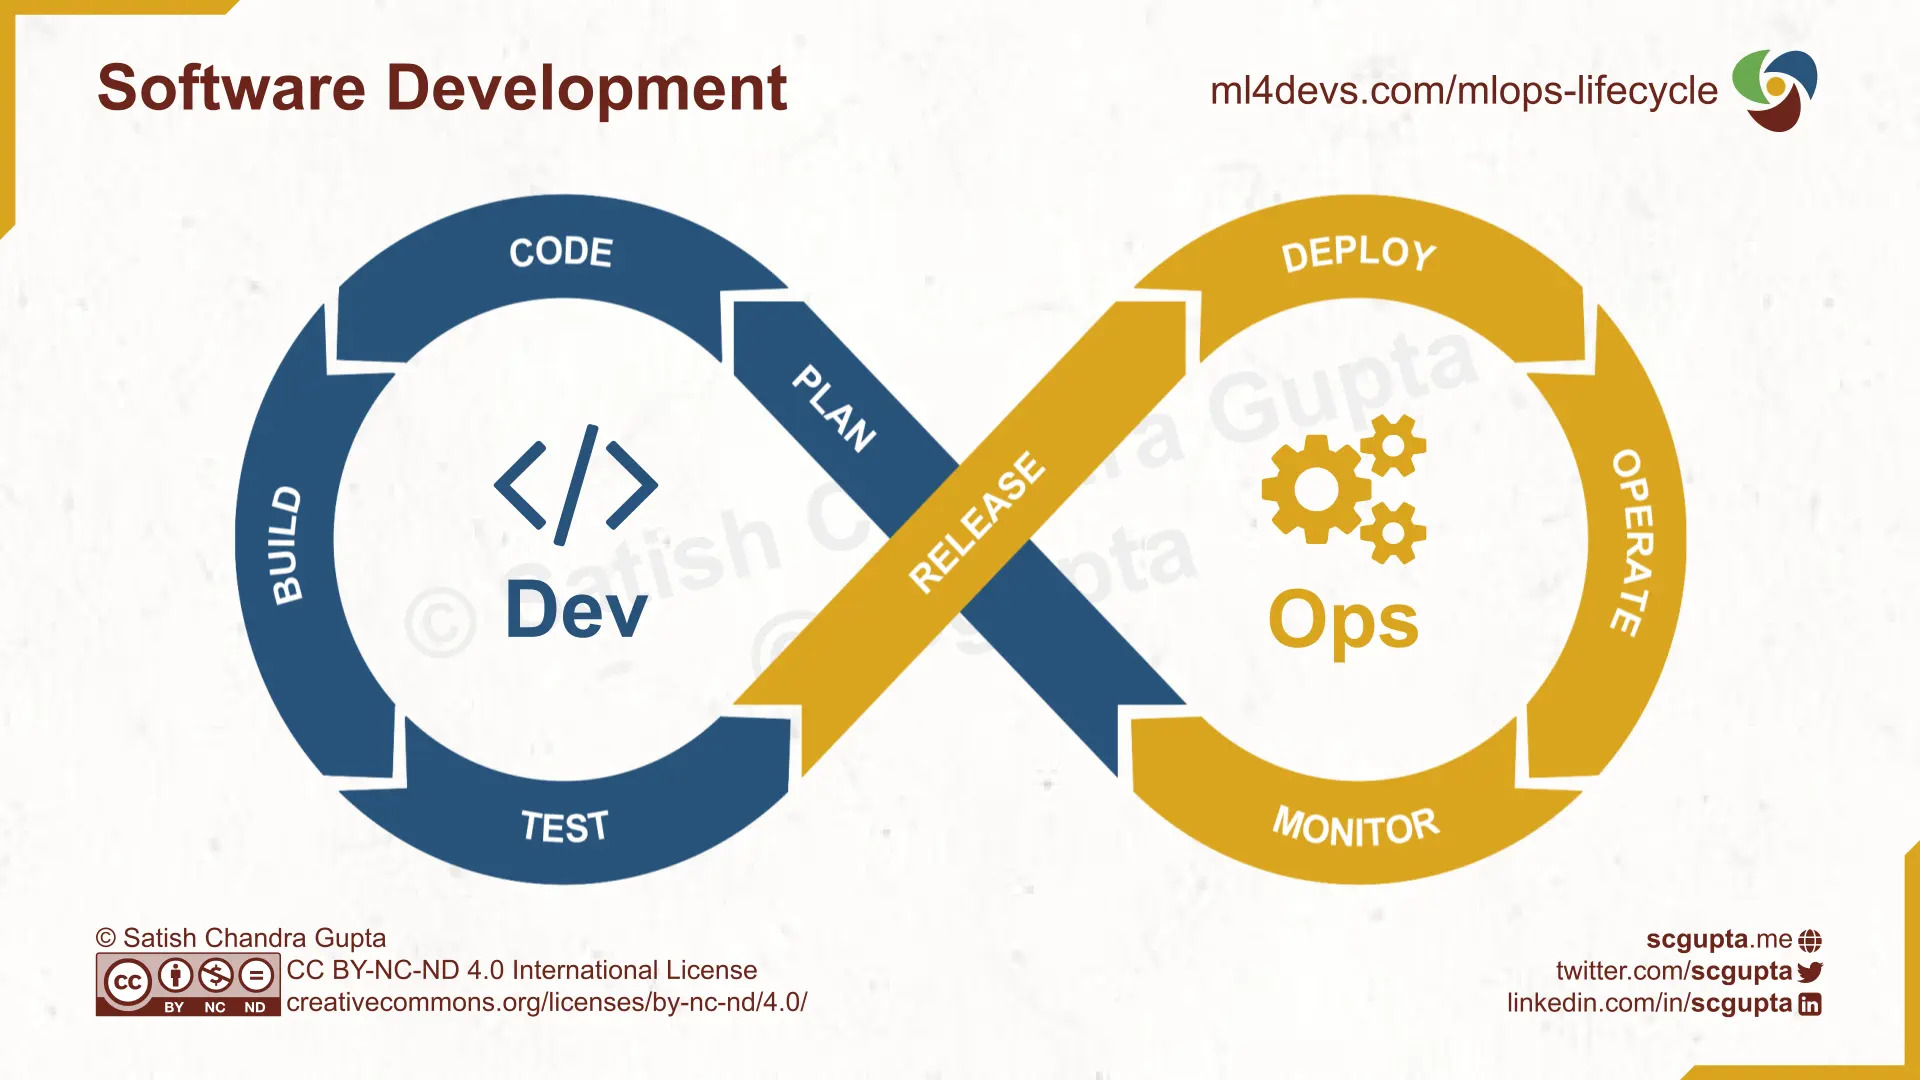
\includegraphics[width=.8\textwidth]{devopsmodel.jpeg}
\caption{Software Development Lifecycle}
\label{fig:devopsmodel}
\end{figure}

The lifecycle in Figure~\ref{fig:devopsmodel} begins with planning the software application, defining what the application is required to do, its users, its business objective, etc. Software developers then produce programming code. The build phase integrates the separate code pieces from all developers into a complete application, and from this builds the actual software application in the development environment. The test phase moves the software application to a testing environment. It conducts functional tests to ensure the application works correctly, but also performs security tests and performance tests to ensure it poses little risk and consumes reasonable resources. An application is then formally released into production. Resources such as hardware, databases, file storage space, network connections, etc. are provisioned, forming the production environment. The application is then deployed into its production environment, integrated with other software applications and operated. Continuous monitoring ensures the software applications continues to work, to work correctly, and to consume only the anticipated resources. The analysis of monitoring data will lead into a new iteration of the DevOps lifecycle where the next version of the application is planned, developed, and operated.

The combined lifecycle model in Figure~\ref{fig:mlopslifecycle} recognizes the fact that machine learning models are just one part of a complex software application. Consider the example of the dynamic pricing web-store application. The actual prediction model, while central and important, is but a small part of it that must integrated into the web-store application. When the available training data changes (in the ''collect'' phase), all phases of the lifecycle may need to be performed again to create a new model, develop or adapt the software application and move it to operations. Given the number of steps involved and their complexity, it becomes clear that managing this lifecycle efficiently, and managing it at scale for multiple models, requires formalized and automated processes.

\begin{figure}
\centering
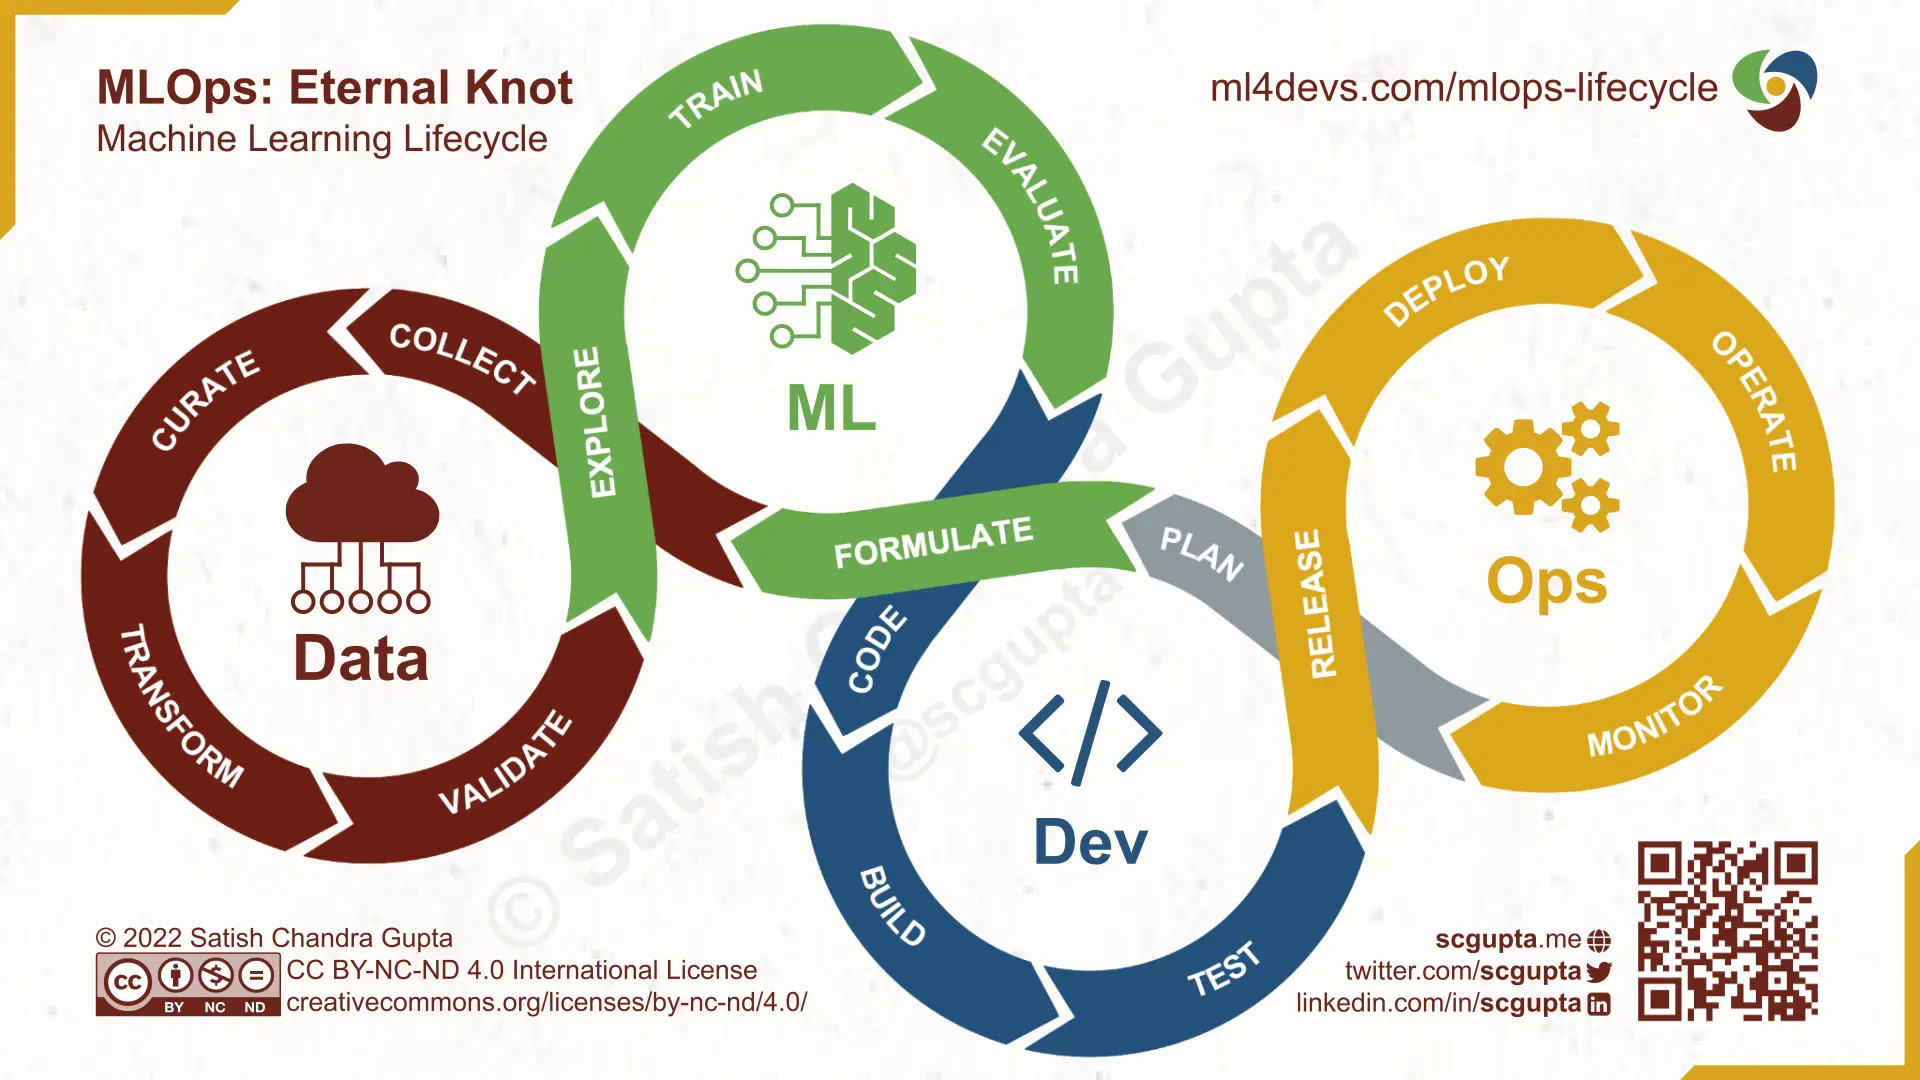
\includegraphics[width=\textwidth]{mlops2.jpeg}
\caption{MLOps Lifecycle}
\label{fig:mlopslifecycle}
\end{figure}

\FloatBarrier

\section{MLOps Roles and Requirements}

Many people participate in different roles in MLOps processes. They participate in or take responsibility in different phases of the overall MLOps lifecycle, as shown in Figure~\ref{fig:mlopsroles}. This figure shows a simplified representation of the MLOps lifecycle in just 4 phases that are further explained in Section~\ref{sec:mlopslifecycle} below. Each role in the MLOps lifecycle also has certain requirements in order to perform the role efficiently.

\paragraph*{Subject matter experts} are business stakeholders that provide the business problems, questions, or goals for a machine learning project. They also define how the success of a project will be measured in business terms by defining the relevant KPIs (key performance indicators). In a dynamic pricing example, a business KPI might be to improve the acceptance rate of customized product offers by 5 percent. These KPIs inform the choice of model and of model evaluation metrics. Once the model is in production, subject matter experts evaluate the performance against the business needs, that is, the KPIs. This evaluation cannot be done by the MLOps team, because it concerns the business goals, not the predictive performance of a model: The model may perform well in predicting the price customers are willing to pay, but customers for other reasons choose not to accept product offers.

Subject matter experts require understandability and interpretability of models, if they are to assess them in business terms. Moreover, they require a responsive feedback mechanism so that their evaluations and assessments can inform the next iteration of the MLOps lifecycle.

\begin{figure}
\centering
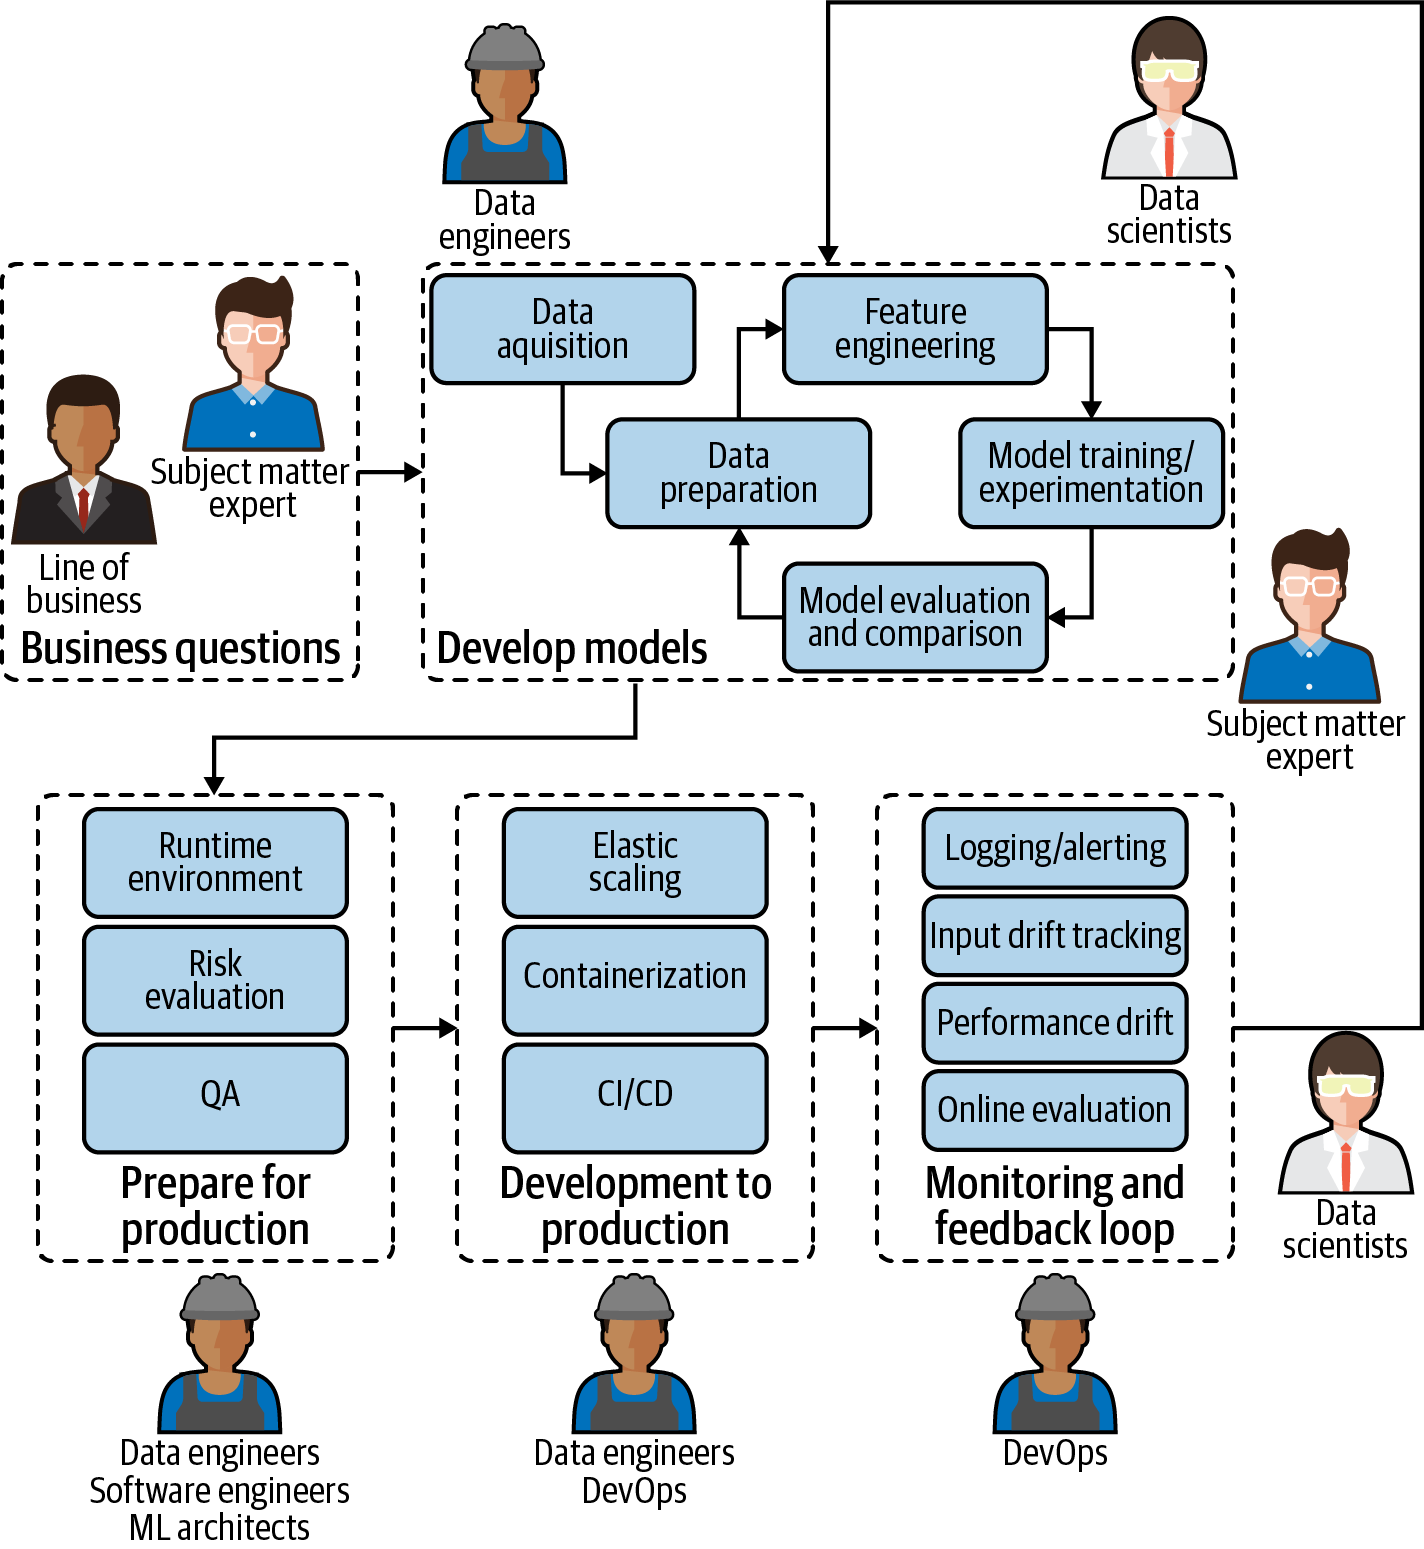
\includegraphics[height=3.25in]{imlo_0103.png} \\

\scriptsize \textbf{Source:} Treveil et al. (2020), Figure 1-3
\caption{Roles in the MLOps lifecycle}
\label{fig:mlopsroles}
\end{figure}

\paragraph*{Data scientists} use available data sets to develop, train, and evaluate different machine learning models, based on the goals defined by the subject matter experts. Their tasks also include related activities such as data preprocessing and feature engineering that are necessary for training and evaluation. 

\paragraph*{Data Engineers} work with data scientists to acquire or collect, manage, clean, maintain, and provide data. They build the data infrastructure necessary for data scientists to efficiently access the data during model training and evaluation. This includes providing file storage space or databases or data warehouses. Data engineers are also involved in data acquisition from internal or external sources, in evaluating and maintaining data quality and in maintaining data provenance.

To perform their tasks efficiently, data scientists and data engineers require automated model packaging and delivery tool. That is, once a model has been developed and found to be have acceptable performance, packaging the model (that is, the trained parameter values, hyper-parameter values, model architecture, training data provenance and description, required software packages, etc.) so that it can be moved to production deployment should be automatic. Data scientists and data engineers also require automatic testing for models. That is, once a model has been trained, it should automatically be subjected to a variety of tests, from simple predictive performance testing on a range of metrics, through sensitivity testing for a range of normal and abnormal inputs, to interpretability testing. 

Data scientists and data engineers require visibility into model performance as the model moves across the development, staging or preparation, and deployment or production phases. That is, they require access to raw performance data but better still, access to online visual dashboards for each model or a set of models. They also require visibility into the data pipeline that is used for each model.

\paragraph*{Software Engineers} integrate trained and operationalized models into the software applications of an organization. This can take different forms depending on the nature of the software application. For example, a trained model could be integrated into a mobile application, or it could be accessed as a separate service from the organization's web-based store front. They are supported and advised by data engineers and ML engineers or architects in identifying the most efficient way to deploy and deliver the model within the organization's software applications. 

Software engineers require programming code versioning systems (such as git or GitHub) to collaborate and track the changes that each member of a team makes to the application's code. They also require automatic testing tools for the software application so that, as they make changes to an application's programming code, their changes can be automatically tested locally for correctness and functionality (unit tests) and in the large for compatibility with other changes made by the team (integration tests). 

\paragraph*{DevOps Engineers} are responsible for building the system developed by the software engineers and testing them for security, performance, resource use, failure and fault tolerance, and for availability. DevOps engineers perform the CI/CD processes for continuous integration and continuous delivery of software applications through programming code integration, software building, software testing, to software deployment. 

DevOps engineers require seamless and automatic deployment pipelines, from software code integration, to final testing, infrastructure provisioning (for example, virtual machines, servers, containers, etc.) to deployment into production. In particular, the MLOps lifecycle should integrate at this point with DevOps lifecycle that may already exists in the IT department of an organization and leverage existing processes and tools. 

\paragraph*{Model risk managers and model auditors} are responsible for assessing all types of model risks and ensuring compliance with internal or external regulations and requirements. They assess the models that are developed by data scientists before they move into production. They also monitor the performance of models that are in production to identify relevant changes to the model risk. 

Model risk managers require automated reporting on all models (past and present), including data provenance and all model test results.

\paragraph*{ML Engineers and ML Architects} provide advice on how best to deploy a set of models, the infrastructure required, and the implications of the types of model deployment to software applications. They work closely with data scientists and data engineers who provide knowledge of the model and its data requirements. They make large-scale architectural decisions, such as whether to deploy the model in cloud-based environments like Amazon Web Services or Microsoft Azure, or on-premises, for example using a Kubernetes cluster, or in a web browser or mobile application. They determine scalability and infrastructure requirements.

ML engineers require the ability to easily assess and to quickly adjust infrastructure capacities. For example, if an ML engineer realizes that a ML prediction service performs slowly, the engineer must be able to quickly allocate more servers, deploy additional copies of the ML model, and make them available to the organization's software applications that use that prediction model. 

\begin{figure}
\centering
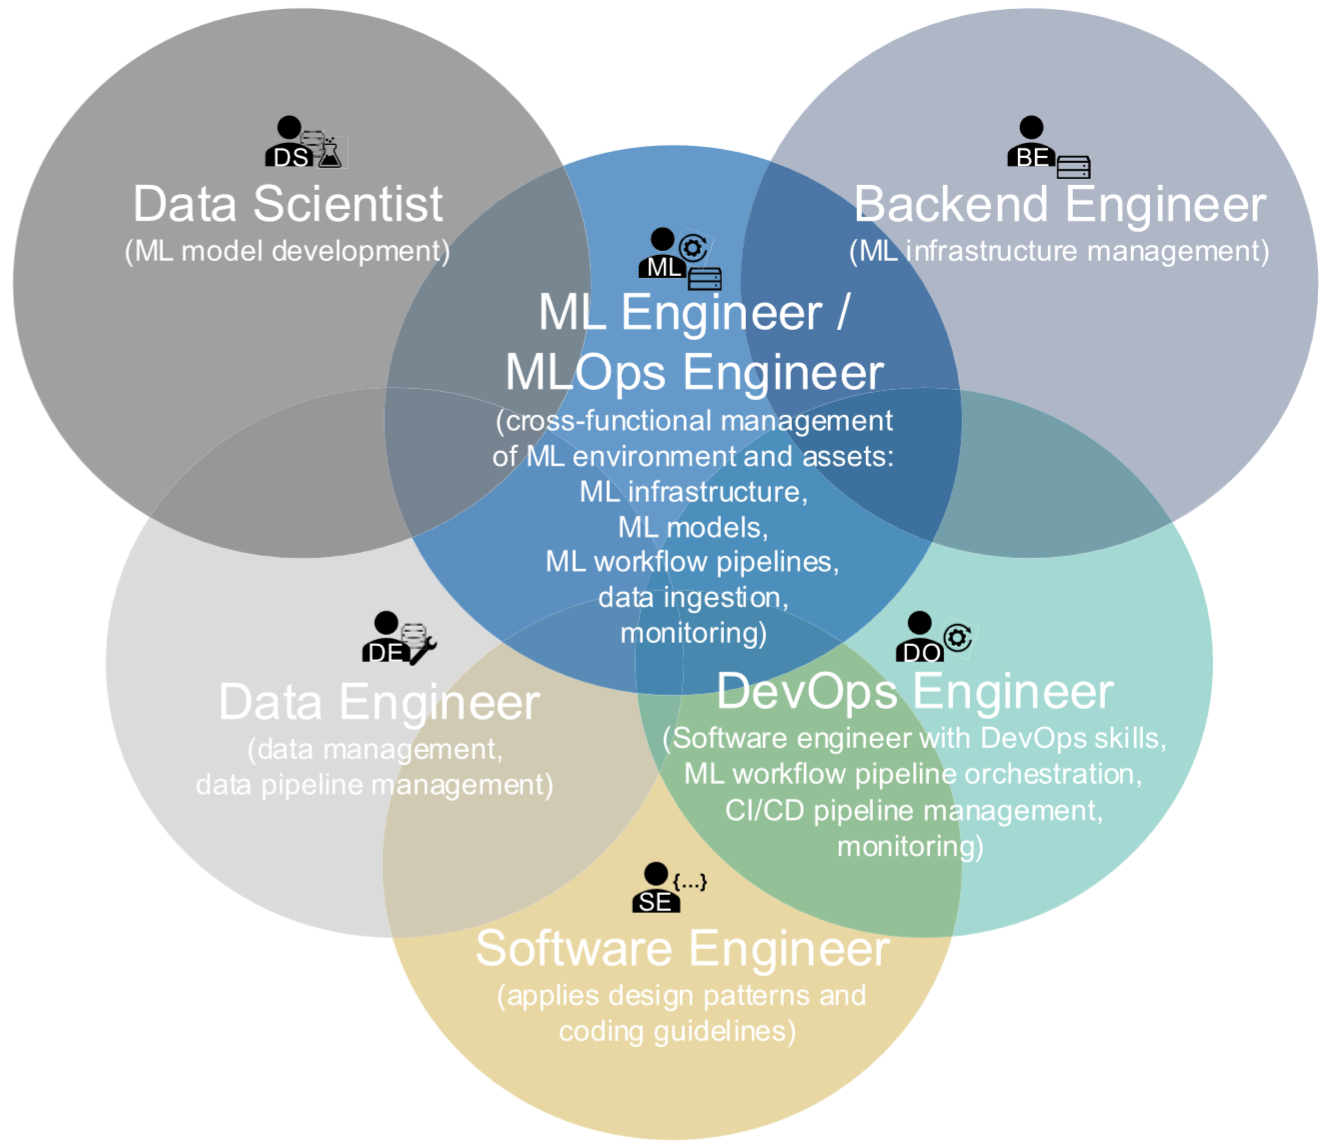
\includegraphics[width=.75\textwidth]{Kreuzbergeretal_fig3.png}  \\

\scriptsize \textbf{Source:} \href{https://ieeexplore.ieee.org/abstract/document/10081336}{Kreuzberger, D., K\"uhl, N., \& Hirschl, S. (2023). Machine learning operations (mlops): Overview, definition, and architecture. IEEE access, 11, 31866-31879.}
\caption{Overlapping MLOps Roles}
\label{fig:mlopsskills}
\end{figure}

\paragraph*{Backend Engineers} provide and manage the computational infrastructure. They create and maintain on-premises or cloud-based computer clusters and distributed storage systems. They design and manage fast and efficient network connections between all components, provide backup and restore functionality, and are responsible for high availability of all infrastructure components. Backend engineers are not included in Figure~\ref{fig:mlopsroles} but are shown in Figure~\ref{fig:mlopsskills} which is taken from a different source.

\section{MLOps Tooling}

Because of its heavy focus on automation, MLOps requires a variety of software tools to support it. This section describes important types of software tool and provides references to some popular examples.

\paragraph*{Source Code Management (SCM), Code Versioning and Code Repositories} are tools that are used by software engineers to collaborate on the creation of a large software application. These tools keep track of all changes and ensure that developers do not overwrite each other's work. The most popular cloud-based tool GitHub\footnote{\url{https://github.com}} is based on the open-source git system\footnote{\url{https://git-scm.com/}}, but many others exist, both open-source and commercial, cloud-based or on-premises. 

\paragraph*{CI/CD} tools are used to integrate software application programming code, automatically build the software system, test it in a test environment, and then deploy it into a production environments. Popular tools of this type are the open-source Jenkins system\footnote{\url{https://www.jenkins.io/}} and GitHub actions\footnote{\url{https://github.com/features/actions}} on the popular GitHub cloud-based platform.

\paragraph*{Workflow Orchestration} tools define the usage of data, model, software and configuration artifacts through the development, test, and deployment cycle. They coordinate data extraction, model training, model inference/prediction, and model or software deployment. A popular open-source on-premises system is Apache Airflow\footnote{\url{https://airflow.apache.org/}}, while AWS SageMaker\footnote{\url{https://aws.amazon.com/sagemaker/}} and Azure Pipelines\footnote{\url{https://azure.microsoft.com/en-us/products/devops/pipelines}} are popular cloud-based tools. 

\paragraph*{Feature Stores} offer centralized storage and management of data and any engineered features for ML models. They track feature updates and changes, assess and monitor data quality, and quickly provide data at training or at prediction time. Popular tools are the open source system Feast\footnote{\url{https://feast.dev/}}, the AWS SageMaker Feature Store\footnote{\url{https://aws.amazon.com/sagemaker/feature-store/}} or Tecton\footnote{\url{https://www.tecton.ai/}}

\paragraph*{Model Training} tools support the definition, training, evaluation and comparison of ML models. They are open-source tools like R, Scikit-Learn, TensorFlow, or Spark, or integrated cloud-based offerings such as AWS SageMaker\footnote{\url{https://aws.amazon.com/sagemaker/}} or Azure Machine Learning \footnote{\url{https://azure.microsoft.com/en-ca/products/machine-learning}}. 

\paragraph*{Model Registries} provide storage for trained models and their meta-data. This includes the model itself, evaluation results, hyper-parameters, training history, data provenance, documentation, and many other artifacts. These tools provide centralized storage, secure access, version management, and other features. They allow model versions to be tracked and to be quickly deployed in the MLOps lifecycle. A popular open-source model registry is MLFlow\footnote{\url{https://mlflow.org/}} while the major cloud platforms also provide model registries, for example the AWS SageMaker Model Registry\footnote{\url{https://docs.aws.amazon.com/sagemaker/latest/dg/model-registry.html}} or the Azure ML Model Registry\footnote{\url{https://learn.microsoft.com/en-us/azure/machine-learning/how-to-manage-models}}.

\paragraph*{ML Metadata Stores} store meta data about MLOps pipeline executions, model training, model lineage, etc. For example, they track when a model was trained, evaluated, packaged for production, moved into deployment, etc. These tools support the auditability and traceability of models and their deployment, in turn supporting risk management and compliance assurance.

\paragraph*{Model Serving} tools execute the model in its production environment and provide access to model predictions or model explanations for the organization's software applications. Popular tools are WSGI\footnote{\url{https://en.wikipedia.org/wiki/Web_Server_Gateway_Interface}} servers such as Flask\footnote{\url{https://flask.palletsprojects.com/en/3.0.x/}}, that are often deployed in containers, TensorFlow Serving\footnote{\url{https://www.tensorflow.org/tfx/guide/serving}}, TensorFlow Lite\footnote{\url{https://www.tensorflow.org/lite}} or TensorFlowJS\footnote{\url{https://www.tensorflow.org/js}} for TensorFlow models, or AWS SageMaker Endpoints\footnote{\url{https://docs.aws.amazon.com/sagemaker/latest/dg/realtime-endpoints.html}} for the AWS cloud platform. 

\paragraph*{Model Monitoring} tools can monitor both the computational performance as well as the prediction inputs and outputs of deployed models. Cloud-based examples are the AWS SageMaker model monitor\footnote{\url{https://docs.aws.amazon.com/sagemaker/latest/dg/model-monitor.html}} on the AWS platform or the Azure ML model monitor\footnote{\url{https://learn.microsoft.com/en-us/azure/machine-learning/concept-model-monitoring}}. 

As MLOps is a relatively young discipline, tool support, both open-source, commercial, and cloud-based, is still evolving rapidly. Figure~\ref{fig:mlopstooling} shows a (partial) overview of companies that offer products and services in this space. Because of the rapid evolution of offerings in MLOps it is simply not possible to provide a detailed description or even a meaningful introduction to these software tools that would remain relevant for more than a few months. 

\begin{figure}
\href{https://mattturck.com/wp-content/uploads/2021/12/2021-MAD-Landscape-v3.pdf}{
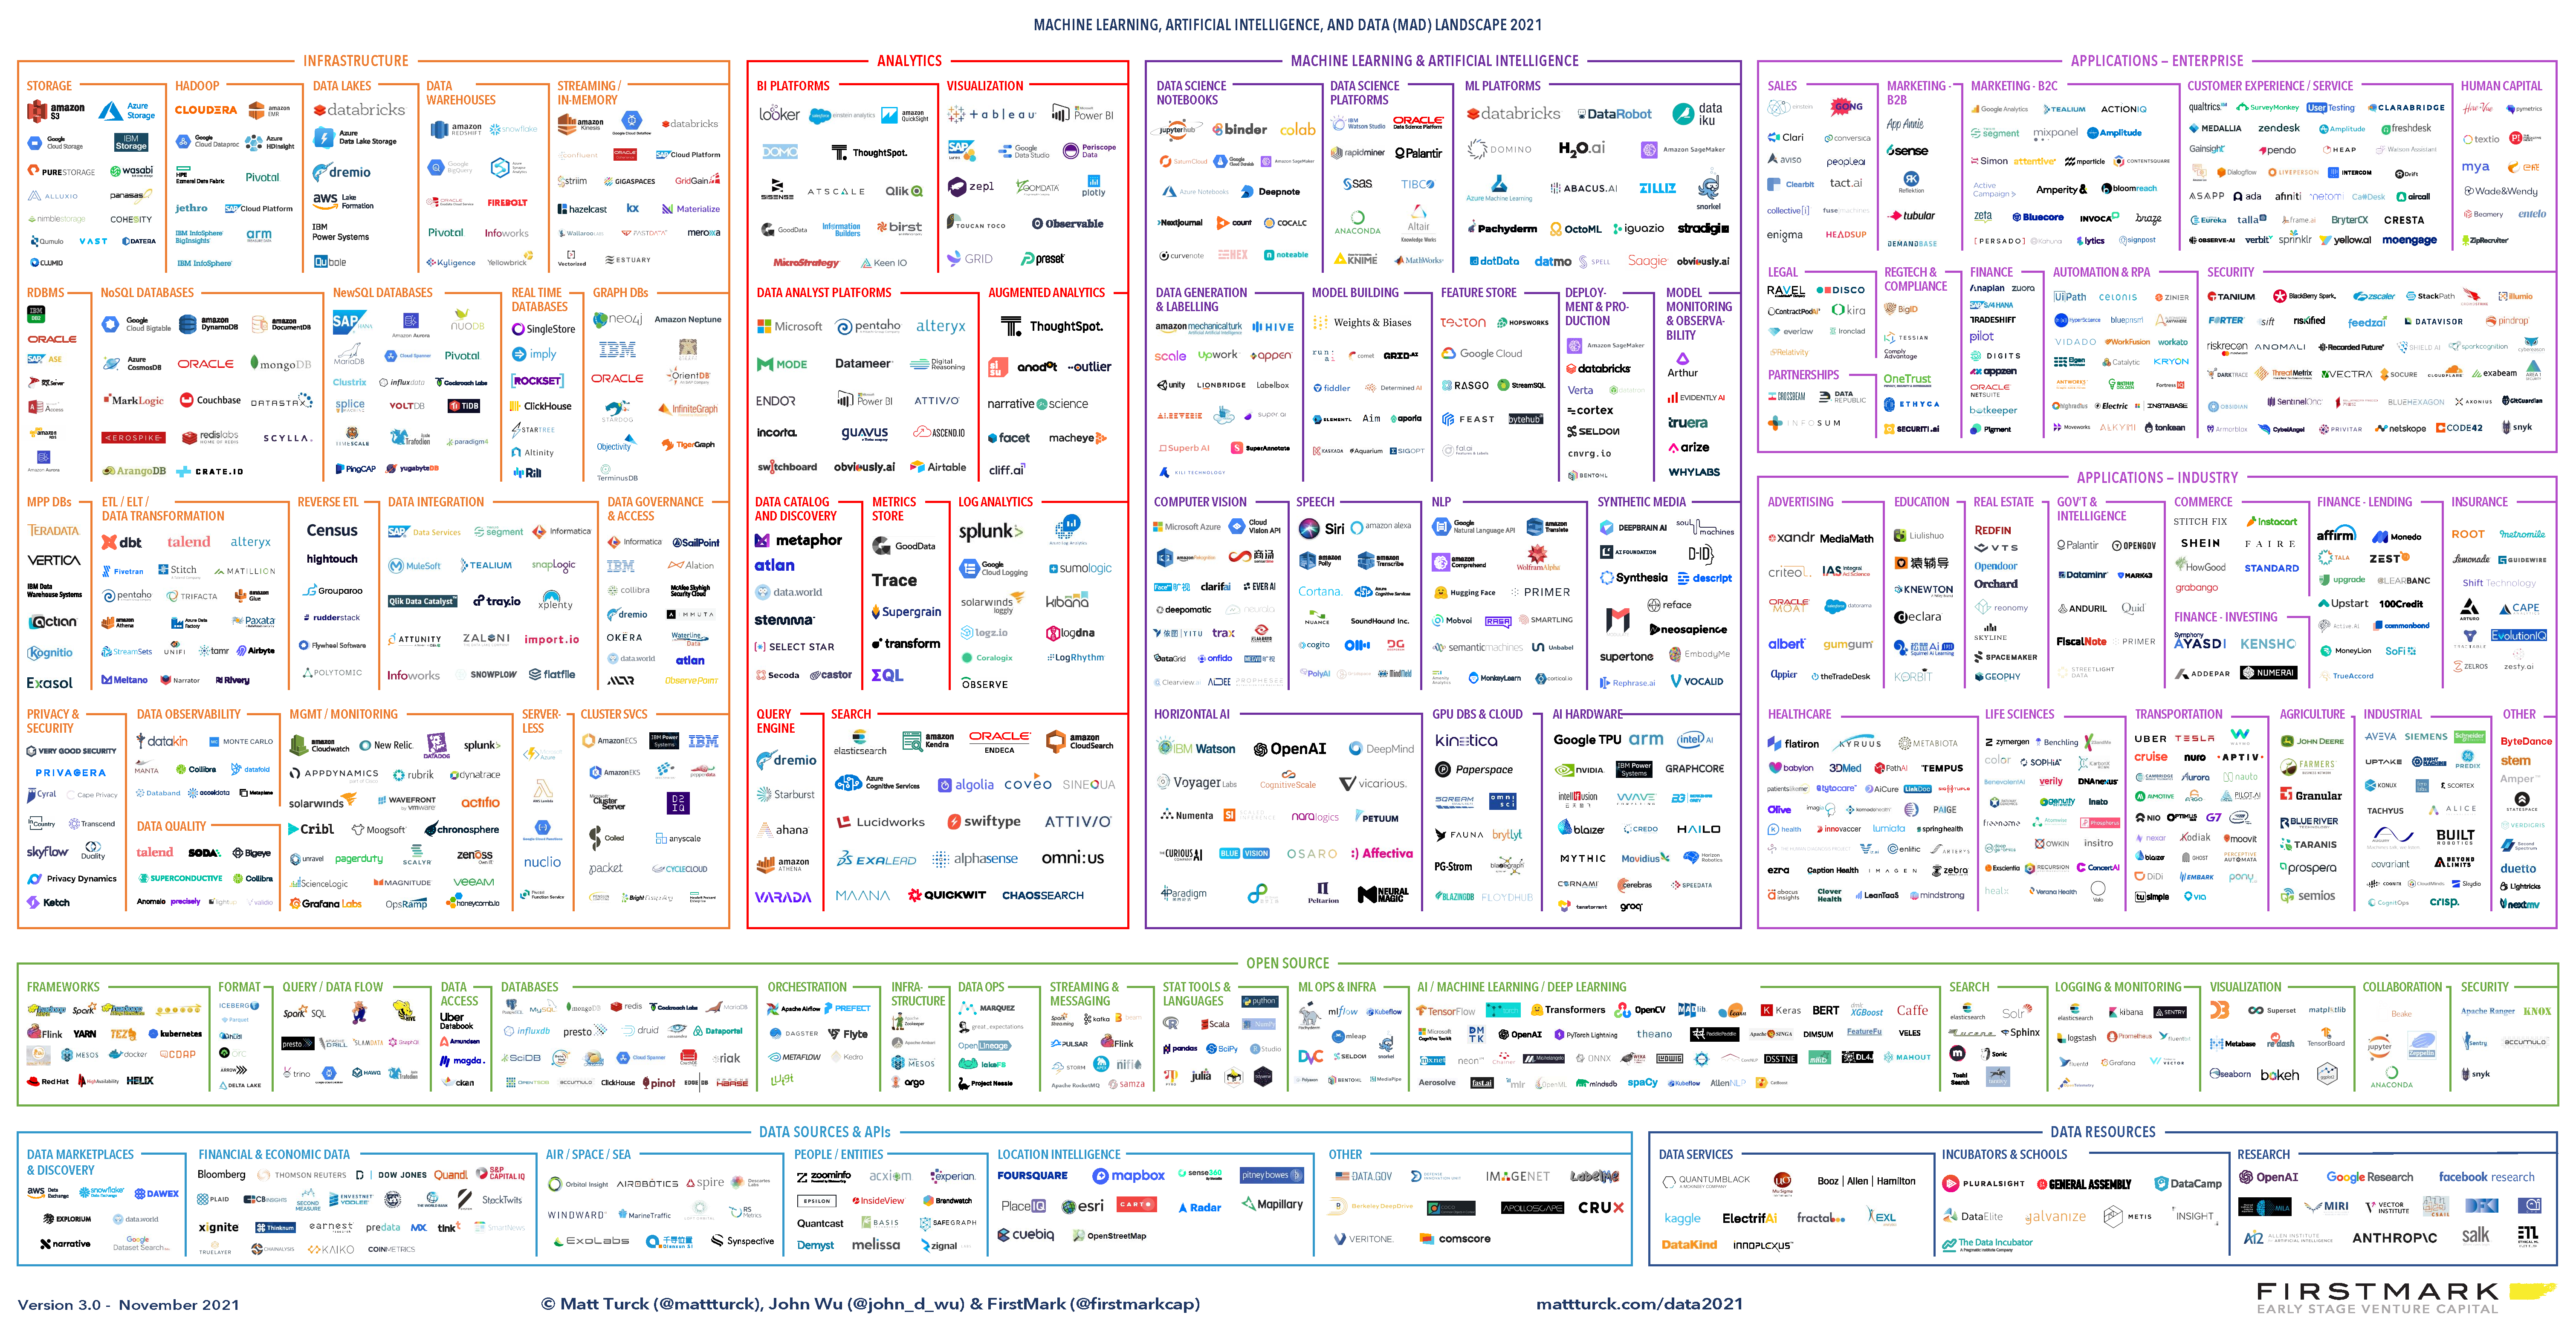
\includegraphics[width=\textwidth]{2021-MAD-Landscape-v3.pdf}} \\

\scriptsize Source: Turck, Matt. \textit{Red Hot -- The 2021 Machine Learning, AI and Data (MAD) Landscape}. September 28, 2021. \url{https://mattturck.com/data2021/} (last accessed July 22, 2024)
\caption{Commercial Offerings in the ML Landscape}
\label{fig:mlopstooling}
\end{figure}

\FloatBarrier
\section{MLOps Lifecycle Phases}
\label{sec:mlopslifecycle}

Figure~\ref{fig:mlopssimplifiedcycle} shows a simplified MLOps lifecycle together with ML governance. While the MLOps lifecycle concerns operations and management, ML governance refers to the oversight and risk management of the MLOps lifecycle and its processes, participants, and tools. The lifecycle in Figure~\ref{fig:mlopssimplifiedcycle} is an abstracted version of the lifecycle underlying Figure~\ref{fig:mlopsroles} above. This section provides brief additional comments on each phase in this simplified lifecycle. 

\begin{figure}
\centering
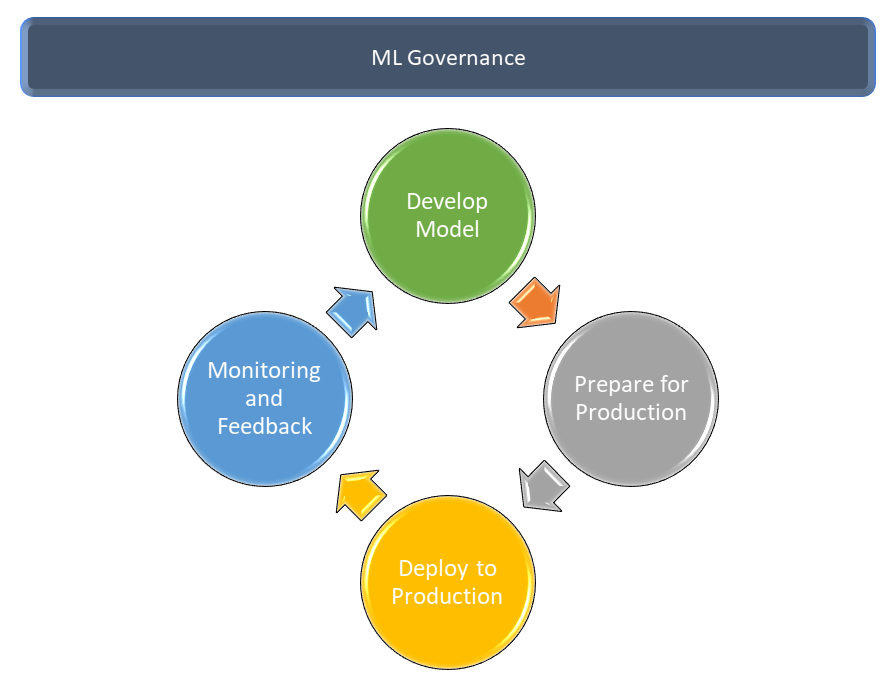
\includegraphics[height=2.5in]{graphics2.png} \\
\caption{Simplified MLOps Lifecycle and ML Governance}
\label{fig:mlopssimplifiedcycle}
\end{figure}

\FloatBarrier
\subsection{Develop Models}

The first phase of the simplified lifecycle, develop models, is highlighted in Figure~\ref{fig:developmodels}. It comprises data and feature engineering, as well as model building, training, evaluation, and comparison. The inputs are training data and other models for comparison (e.g. alternative model types, alternative architecture, the current production model, etc.). The output of this phase are a selected model and its performance metrics and associated documentation. 

\begin{figure}
\centering
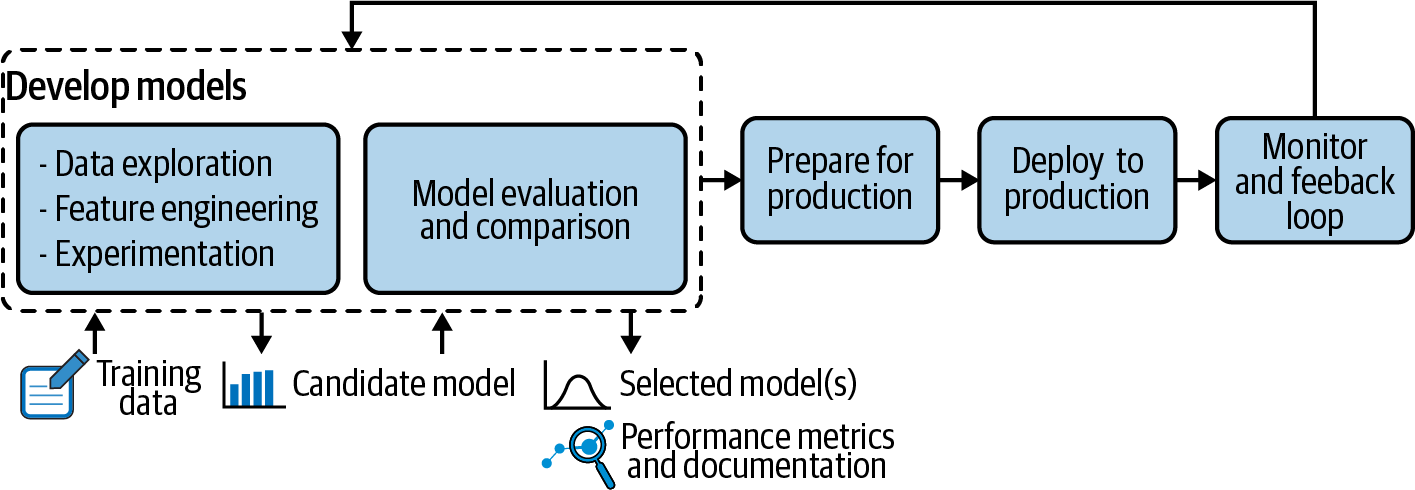
\includegraphics[width=.75\textwidth]{imlo_0401.png} \\

\vspace{\baselineskip}
\scriptsize \textbf{Source}: Treveil et al. (2020), Figure 4-1
\caption{Model development in the MLOps lifecycle}
\label{fig:developmodels}
\end{figure}

From the data management perspective, important questions to ask and answer in this phase are about data permission or licenses, access requirements, and legal or regulatory obligations or constraints. These are questions that help assess the risk and to assure compliance. Specific example questions are:

\begin{itemize}
   \item What data are available? What is the quality of that data?
   \item Can the data legally be used for this purpose? What are the terms of use of the data? What licenses are available or in place for using the data? What is the cost of any required licenses?
   \item How can the data be accessed? Is it available via an external service or does it exist on-premises? What is the technical access mechanism?
   \item What features can be created by combining multiple data sets?
   \item Must the data be redacted or anonymized? Does it include personally identifiable data, such as names or addresses? Does it include sensitive data, such as medical or financial information?
   \item Are there features that cannot be used legally (age, gender, race, etc.) for some purposes? For example, while age and gender could be used in a dynamic pricing application, they are not legally useable in many jurisdictions for evaluating job applications or making hiring decisions. 
   \item Is the data representative of minority classes/populations? When the data set is biased towards a large majority class or only covers part of the target population, a predictive model built from it will not perform well for minority classes. At best, this increases the risk due to poor predictions, at worst, this prohibits the use of the model in some jurisdictions as it may not exhibit fairness towards all classes or sub-populations.
\end{itemize}

Tool support for data management in this phase includes ETL pipelines to extract data from source systems, transform it, and load it into a central data or feature store. It also includes centralized data storage, feature storage, and feature engineering tools. 

From the model management perspective, important questions also address bias and fairness of model predictions or outcomes. Again, this is to assess and mitigate model risk and to ensure compliance with regulatory and legal obligations. Specific questions to ask include the following:

\begin{itemize}
   \item What are appropriate evaluation metrics? How do these metrics relate to the business KPIs and the goals of the model?
   \item Is the model performance acceptable globally and for different sub-populations? How are different performance metrics, such as precision and recall, combined into an overall model performance assessment?
   \item Does the model need to be interpretable or explainable? What type of explanations, for example global or local, should be provided to the model user? 
   \item Are the model outcomes fair to all possible users? How is fairness defined? Are there conflicting definitions or requirements for fairness and how are they combined and reconciled?
\end{itemize}

Tool support for model definition and management include model registries and repositories that can keep track of and store the models themselves (trained parameters), but also the hyper-parameters, random seeds, software versions, train and test histories and results, associated documentation, etc. Feature stores are used at this stage to provide the data for model training and container makefiles and container registries are often used to provide fixed and reproducible training environments, including all required software packages in their specific versions.  

\subsection{Prepare for Production}

Preparing a model for production, highlighted in Figure~\ref{fig:prepareforproduction}, includes selection of the runtime environment and deployment mode (e.g. as a micro-service, as a model embedded in a mobile app, etc.). This decision is made by ML engineers in collaboration with data engineers and data scientists. Preparing for production involves risk assessment of the model and quality assurance of the model by model risk managers and model auditors. Risk mitigation measures are put into place (e.g. an automatic fail-safe when out-of-scope inputs are detected), the model security is tested and improved if necessary, and reproducibility and auditability of the model are confirmed. 

\begin{figure}[h]
\centering
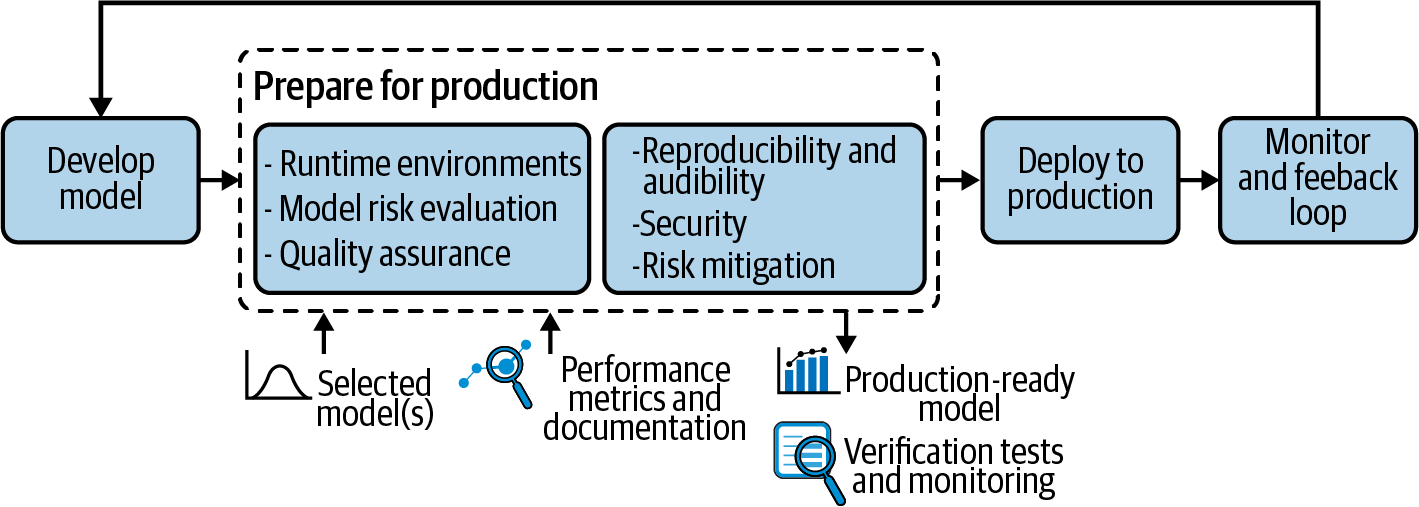
\includegraphics[width=.75\textwidth]{imlo_0501.png} \\

\vspace{\baselineskip}
\scriptsize \textbf{Source}: Treveil et al. (2020), Figure 5-1
\caption{Prepare for Production in the MLOps Lifecycle}
\label{fig:prepareforproduction}
\end{figure}

The input to this phase are the selected model together with its performance metrics and associated documentation. The output is a production ready model with the results of the verification tests performed during this phase. 

Technical questions to ask and answer and decisions about the runtime environment to be made during this phase include the following:
\begin{itemize}
   \item What is the runtime environment and deployment mode? Example options are WSGI services in containers deployed on clusters (on-premises or cloud-based), TensorFlow Serving deployment (again, either on-premises or cloud-based), so-called ''edge-devices'' such as mobile phones, embedded systems or IoT devices (internet-of-things), or in a web-based application as a JavaScript model.
   \item Does the model need to be adapted for production? For example, quantization can increase the performance of model predictions significantly by replacing large floating point numbers with smaller ones. Often, models are trained with 32 bit floating point numbers, but then deployed with 8 bit numbers. The loss in precision may be negligible while the performance benefits can be significant. Another example of model adaptation is additional pruning of decision trees. Again, careful pruning may have a negligible impact on prediction accuracy but a significant impact on prediction performance. 
   \item How are data features accessed or provided? For example, a prediction model that includes as a feature the customer's driving distance to the business location requires a service that can calculate this distance from a given address at the time of prediction (at ''inference'' time or at ''run'' time). A prediction model that includes the weather or temperature of a given day requires access to a service that can provide this information at run time. Such services need to be internally or externally provisioned, licensed and potentially paid for. 
\end{itemize}

To assess model risk, relevant questions to ask by the model risk manager include the following:
\begin{itemize}
    \item What can happen if the model acts in the worst possible way? What is the worst possible error of the model and what are the financial, business, legal or reputational impacts when the model behaves in such a way? What is the legal liability for decisions that are made based on such model behaviour?
    \item What if a client extracts training data or model details? For example, consider a KNN model where $k$ is very small, e.g. 2 or 3. With just a few observations, and the prediction of the model, other observations in the training set could be identified or deduced. 
    \item What are financial, business, legal, and reputational risks? Who assumes liability for model errors and can the liability be reduced? Are there legal implications for model errors? Are there reputational risks? The extent of such risks and the impact of model prediction error differs from use case to use case. For example, in large-scale medical diagnostics, the impacts may be much more severe than in a small pilot implementation of a dynamic pricing application. 
\end{itemize}

Sources of risk that a model risk manager or model auditor should consider include the following:

\begin{itemize}
   \item \emph{Errors in model design or training}: Is the appropriate model type chosen? Is the model architecture appropriate to the problem and are the hyper-parameters chosen well? Did model training use the data correctly and use the correct data?
   \item \emph{Errors in the runtime environment}: Are there security flaws or security ''holes'' in any of the software packages that are used in the runtime environment? Are there known limitations of the packages for certain situations and do they affect the deployed model?
   \item \emph{Data quality problems}: Was the training data of sufficient quality? Were data transformations and data pre-processing carried out correctly and verified?
   \item \emph{Differences between training \& production data (''input drift'')}: Over time, the characteristics of the input data may change. For example, future customers may be different from past customers as the business's products, services, competitive position, and strategy evolve. A model that was built based on past customers' training data may no longer provide good predictive performance for current or future customers. 
   \item \emph{Abuse of model or misuse of outputs}: Is the model used only for the purpose it was designed for, or are its outputs also used in other ways? For example, the output of a dynamic pricing model that predicts the maximum amount a customer is willing to pay for product could also be used to offer short-term consumer credit to the customer for that product. However, the willingness to pay a particular price for an item is not the same as the ability to afford to pay a particular price or loan.
   \item \emph{Adversarial attacks}: For example, consider a recommender system that predicts the probability of future movie choices on a streaming platform. Can the system be tricked into recommending age-inappropriate movies when a particular input is provided?
   \item \emph{Legal risk from training data use or model results}: What are the implications of using training data for which permission to use was not obtained? Can the model be easily retrained when customers or third parties withhold or retract permission to use their data.
   \item \emph{Reputational risk}: Some ML model errors are high profile and covered by national and international news outlets. This can have serious implications for the reputation of a company and its relationship with its customers. 
\end{itemize}

Detailed and up-to-date documentation can help the risk manager in objectively evaluating the probability and potential impact when these risks are realized. A number of risk mitigation procedures are available to mitigate the risks, including:

\begin{itemize}
   \item \emph{Shadow testing} of a new model is to deploy both the old and new replacement model at the same time. Both models receive the same inputs but only the old model's predictions are used or served to the client application. This allows testing of a candidate new model on actual production data to ensure it will only go live when it is confirmed to be no worse than the existing old model. Because the new model is already deployed, switching the input and output traffic is then a simple matter.
   \item \emph{Progressive rollout} (sometimes called ''canary deployment'') also uses both an old and a new replacement model. However, rather than shifting input and output entirely from the old to the new model, this is done progressively for increasing proportions of traffic. For example, initially, only 10\% of customer input is routed to the new model. Then, after the model behaviour has been assessed, this is increased to 20\%, etc.
   \item \emph{Continuous logging and monitoring} is important to detect abnormal inputs which can signal an adversarial attack or a software malfunction. Alarms are raised and the model can be taken offline or replaced with a simpler model. Logging and monitoring is also important to detect gradual input drift, that is, changing characteristics of the input data, which indicates that the model is no longer appropriate and should be retrained. 
   \item \emph{Input and output checks} are quick, simple checks that ensure that input values fall within an acceptable range, are of an appropriate data type, etc. For example, a dynamic pricing model may check inputs to ensure that customer addresses are valid and in the business' geographic market. Output checks are common-sense checks that ensure the model predictions are at least sensible. For example, in a dynamic pricing application, the predicted price should be positive and within a range appropriate to the product category that is being priced. 
   \item \emph{Fail-over to simpler model} is the degradation of a model to a simple backup when a model failure occurs. For example, the complex neural network model in a dynamic pricing application may be unavailable because of software errors, adversarial attackes, or invalid input or invalid output. In its place, a simpler linear regression model may be used.
   \item \emph{Periodic retraining} should occur whenever an input drift has been detected or a significant amount of new training data is available. This ensures that the model remains appropriate and useful for its intended purpose.
\end{itemize}

Automation tools used during the preparation for production include continuous integration and automated testing tools for quality assurance and model risk evaluation. Model registries are used during this phase to document all information about a model and document the findings of its quality assurance and risk evaluation, including input data sources and data provenance, model assumptions, required software packages, test results including explanations and bias or fairness evaluations, training and test logs, security test results, etc. 

\subsection{Deploy to Production}

Deploying a model to production includes both the CI/CD (continuous integration/ continuous deployment) pipelines for deploying the software that uses the model as well as building the ML model and related artifacts. The deploy to production phase is highlighted in Figure~\ref{fig:deploytoproduction}. Inputs are a production ready model and completed verification tests. The output is a model in its production environment. 

\begin{figure}[h]
\centering
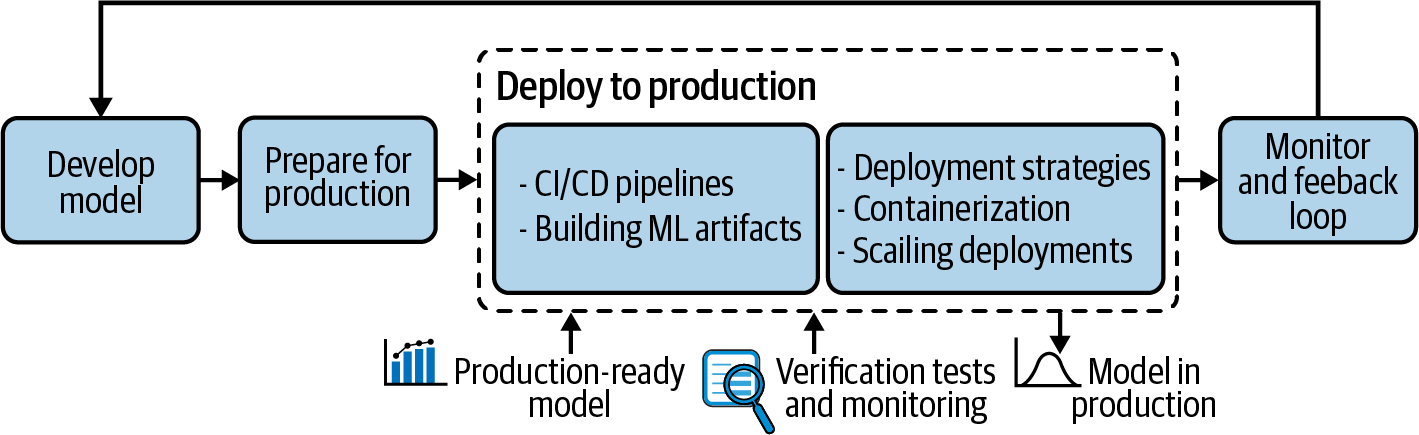
\includegraphics[width=.75\textwidth]{imlo_0601.png} \\

\vspace{\baselineskip}
\scriptsize \textbf{Source}: Treveil et al. (2020), Figure 6-1
\caption{Deploy to Production in the MLOps Lifecycle}
\label{fig:deploytoproduction}
\end{figure}

A typical, automated CI/CD pipelines comprises at least the following steps\footnote{Adapted from Treveil et al. (2020) (pg. 74f)}:

\begin{samepage}
\begin{enumerate}
\item Build model
\begin{enumerate}
   \item Build model artifacts (model code, configuration, data, trained model, environment, documentation, test code and test data)
   \item Archive model on model store and register model with model registry
   \item Basic checks for model
   \item Evaluate bias and interpretability 
\end{enumerate}
\item Deploy to test environment
\begin{enumerate}
    \item Evaluate predictive performance
    \item Evaluate computational performance
\end{enumerate}
\item Deploy to production environment
\begin{enumerate}
   \item Limited deployment (shadow, progressive (''canary'') deployment)
   \item Full deployment
\end{enumerate}
\end{enumerate} 
\end{samepage}

Deployment includes considering the scalability and reliability of the model at  inference time. Deployment targets (that is, server types and numbers) must be chosen that are appropriate to the expected workload. For example, an ML architect must be determine which servers should serve the model predictions, where in the world they should be located, how many there should be, and other technical considerations. Workload balancing for multiple servers must be defined and set up, for example, based on input features, request characteristics such as geographic location, or randomly. Automatic fail-over to replacement servers must be defined. This includes the ability to automatically detect server failure and to automatically re-provision replace servers. This phase must also consider how model upgrades are performed (e.g. shadow deployment, progressive deployment).

Deployment to production also includes defining and provisioning infrastructure for continuous monitoring. Three aspects should be monitored regularly. Resource monitoring measures the infrastructure resources consumed by the model in production. This includes CPU computation time, network traffic, database and file storage space, and many related metrics. Abnormally high or low values can indicate operational problems and must be investigated. Model health checking involves assuring that the model serving software does actually accept prediction requests and provides model predictions. That is, it ensures the software works. This is different from resource monitoring which can only measure whether the server computer is busy. Finally ML metrics monitoring focuses on prediction metrics, such as input and output characteristics or their distributions, or prediction error rates or accuracy (if ground truth is available at that time or shortly after). 

Automation tools required and used during this phase of the MLOps lifecycle include source code repositories such as GitHub and software integration tools such as Jenkins to build and test the model and related software applications. Also required are model registries such as MLFlow and model serving tools such as TensorFlow Serving or Flask. Finally, log data storage and log analysis software is required for monitoring. 

The remainder of this section illustrates two basic deployment methods for a neural network model developed using Keras. As a first step, the model is defined and trained. The following example uses a very simple linear regression model for the Boston housing price dataset. The focus here is not on the quality of the model but on how the trained model can be deployed. 

\begin{tcolorbox}[colback=alert]
\subsubsection*{Resources}
Complete implementations of all examples in this chapter are available in the following GitHub repo:

\url{https://github.com/jevermann/busi4720-mlops} \\

The project can be cloned from this URL:

\url{https://github.com/jevermann/busi4720-mlops.git}
\end{tcolorbox}

As a first step, the data set is retrieved, features are created and the linear regression model is defined\footnote{
Complete implementation is available at \url{https://github.com/jevermann/busi4720-mlops/blob/main/train_model.py}}. \\

\begin{samepage}
\begin{pythoncode}
import keras.utils
import pandas as pd
import tensorflow as tf
import tensorflowjs as tfjs

keras.utils.set_random_seed(42)
boston_data = pd.read_csv("https://evermann.ca/busi4720/boston.csv")

boston_features = boston_data[['rm', 'tax', 'age']]
boston_labels = boston_data['medv']

# Linear regression model
norm_boston_model=keras.models.Sequential([
    keras.layers.Input(shape=(3,), dtype=tf.float32),
    keras.layers.Dense(1, activation=None) ])
\end{pythoncode}
\end{samepage}

Next, the model is trained and saved in three different ways, for use in Keras, for use in TensorFlow serving, and for use in TensorFlowJS. Each of these require a different model package format.

\begin{samepage}
\begin{pythoncode}
stop_callback = keras.callbacks.EarlyStopping()
norm_boston_model.compile(
    loss = tf.keras.losses.MeanSquaredError())
norm_boston_model.fit(
    boston_features, boston_labels,
    epochs=100, validation_split=0.33,
    callbacks=[stop_callback])

# Save model for use in Keras
norm_boston_model.save('norm.boston.model.trained.save')
# Export model for use in TF Serving
norm_boston_model.export('norm.boston.model.trained.export')
# Convert model for use in TFJS
tfjs.converters.save_keras_model(norm_boston_model,
    'norm.boston.model.trained.tjfs')
\end{pythoncode}
\end{samepage}

\subsubsection*{Deployment as a Flask Microservice}

The following code blocks illustrate how a trained model may be deployed as a micro-service using the Flask WSGI server. Flask is a Python package that functions as a web server, accepting requests from client applications over the network and sending an appropriate response. In this example, client applications send the input data for the prediction model as a JSON object in the web request, and the Flask service responds with a JSON object that contains the prediction and other information\footnote{Complete file is available on \url{https://github.com/jevermann/busi4720-mlops/blob/main/flask_deploy.py}}.

First, the saved model is loaded. The \texttt{predict()} function accepts the inputs and provides suitable output (assuming that inputs are single observations, it returns the first and only target of the first and only element of a batch).

\begin{samepage}
\begin{pythoncode}
import keras
import flask
from flask import request
import pandas as pd

# Load the trained model
norm_boston_model = keras.saving. \
    load_model('norm.boston.model.trained.save')

# A predict function for the model
def predict(inputs):
    return norm_boston_model.predict_on_batch(inputs)[0][0]
\end{pythoncode}
\end{samepage}

Setting up the Flask web server is simple. The \texttt{app} defines the Flask application and the decoration \texttt{@app.route(...)} indicates that the \texttt{predict\_json()} function should be called when a client requests the \texttt{/predict\_json} URL using the \texttt{POST} method on the server. The \texttt{predict\_json()} function accepts the input data from the request, and creates a suitable Pandas dataframe. It calls the \texttt{predict()} function and packages the resulting prediction as a JSON object to be returned to the client. 

\begin{samepage}
\begin{pythoncode}
app = flask.Flask(__name__)

# Define the URL handler:
@app.route("/predict_json", methods=["POST"])
def predict_json():
    reply = {}
    # TODO: Input checking goes here
    # TODO: Input logging goes here
    inputs = pd.DataFrame.from_dict(request.json).transpose()
    prediction = predict(inputs)
    # TODO: Output checking goes here
    # TODO: Output logging goes here
    reply["prediction"] = str(prediction)
    reply["success"] = True
    return flask.jsonify(reply)

# Run the server app
app.run()
\end{pythoncode}
\end{samepage}

To access this microservice application when it is running, a simple web request can be used from the Bash command line\footnote{Complete file is available on \url{https://github.com/jevermann/busi4720-mlops/blob/main/json_demo.sh}.}. The \texttt{curl} program sends web requests and receives and prints the responses, the \texttt{-X} option specifies the request method, the \texttt{-H} option specifies request headers, \texttt{--data} specifies the data to be sent and the final argument is the web server address and URL. 

\begin{samepage}
\begin{bashcode}
curl -X POST \
     -H "Content-Type: application/json" \
     --data '[6, 250, 66.5]' \
     http://localhost:5000/predict_json
\end{bashcode}
\end{samepage}

To show how such a service may be used from a web-based application, the following code blocks define a simple HTML form\footnote{Complete file is available on \url{https://github.com/jevermann/busi4720-mlops/blob/main/predict_form_async.html}.}. The form provides input fields for the user to enter the input feature values, and in the document header defines a short JavaScript script that calls the Flask microservice to provide the predicted house price. 

\begin{samepage}
\begin{htmlcode}
<!DOCTYPE html>
<html lang="en">
 <head>
  <meta charset="UTF-8">
   <title>Boston Housing Data Prediction Service</title>
   <script>
    async function predict() {
     // Get the values from the text inputs
     const rooms = parseFloat(document.getElementById('rooms').value);
     const tax = parseFloat(document.getElementById('tax').value);
     const age = parseFloat(document.getElementById('age').value);
     // Make a POST request to the server
     const response = await fetch('/predict_json', {
       method: 'POST',
       headers: { 'Content-Type': 'application/json' },
       body: JSON.stringify([rooms, tax, age]);
     });
     // Parse the JSON response
     const result = await response.json();
     // Display the result
     document.getElementById('output-div').textContent
       = result.prediction;
   }
  </script>
 </head>
\end{htmlcode}
\end{samepage}

The body of the HTML document is the HTML form with its input elements. When the ''submit'' button is pressed, the \texttt{predict()} function defined in the document header in the previous HTML code block is executed. 

\begin{samepage}
\begin{htmlcode}
 <body>
  <h1>Boston Housing Data Inputs</h1>
  <form onsubmit="event.preventDefault(); predict();">
   <p>
    <label for="rooms">Number of Rooms</label>
    <input name="rooms" id="rooms" required>
   </p>
   <p>
    <label for="tax">Tax Rate per 10,000</label>
    <input name="tax" id="tax" required>
   </p>
   <p>
    <label for="age">Prop bldg older than 1940</label>
    <input name="age" id="age" required>
   </p>
   <input type="submit" value="Submit">
  </form>
  <p>Prediction is: <div id="output-div">...</div></p>
 </body>
</html>
\end{htmlcode}
\end{samepage}

The Flask application defined here is typically packaged in container (using Docker or other container technology). One or more instances of such a container are then executed on container servers, depending on the required capacity. Container deployments to servers are typically automatically performed using software such Kubernetes\footnote{\url{https://kubernetes.io/}}, which is an open-source container orchestration system for automating software deployment, scaling, and management. 

\subsubsection*{Deployment as a JavaScript Model}

Another way to deploy an ML model is to embed it in a browser-based web application. This deployment has the advantage that the organization does not need to provide computational resources to run the model at inference time, and the prediction request and response need not be sent across a network connection. On the other hand, this deployment is suitable only for small models and only for models that can be made available to application users as organization loses control over the model and must treat its results as insecure. Examples where such models may be useful could be object recognition tasks in a web browser, speech translation or transcription in a web video conferencing application, etc. 

The following HTML code block\footnote{Complete file is available on \url{https://github.com/jevermann/busi4720-mlops/blob/main/tjfs_demo.html}.} is a slightly altered version of the web form in the Flask example above. Instead of requesting a prediction from the Flask service, the JavaScript scriptloads the model directly using the \texttt{tf.LoadLayersModel()} function provided by the TensorFlowJS framework and calls its \texttt{predict()} function. The document body that defines the form and its input fields is identical to the one in the code block above. 

\begin{samepage}
\begin{htmlcode}
<!DOCTYPE html>
<html>
 <head>
  <script src="https://cdn.jsdelivr.net/npm/\
     @tensorflow/tfjs@latest/dist/tf.min.js"></script>
  <script>
   async function predict() {
    // Load the model
    const model = await \
     tf.loadLayersModel('https://raw.githubusercontent.\
      com/jevermann/busi4720-mlops/main/model.json');
    // Get the values from the text inputs
    const rooms = parseFloat(document.getElementById('rooms').value);
    const tax = parseFloat(document.getElementById('tax').value);
    const age = parseFloat(document.getElementById('age').value);
    // Package the values into a Tensor
    const inputs = tf.tensor2d([rooms, tax, age],[1, 3]);
    // Get the prediction from the model
    document.getElementById('output-div').innerText = 
     model.predict(inputs).dataSync();
   }
  </script>
 </head>
\end{htmlcode}
\end{samepage}

\subsection{Monitoring and Feedback}

The monitoring and feedback phase of the MLOps lifecycle, highlighted in Figure~\ref{fig:monitoringfeedback}, is important to ensure that the model performance does not diminish or degrade over time. It also detects any input drift, that is, systematic changes in the characteristics or frequency distributions of the input values, and provides a feedback loop for subject matter experts.

Inputs to this phase are the model logs, the ground truth, and developmental data for the deployed model. Ground truth denotes the actual, true value for the predicted target. Output of this phase are metrics that quantify input drift and model performance. 

\begin{figure}
\centering
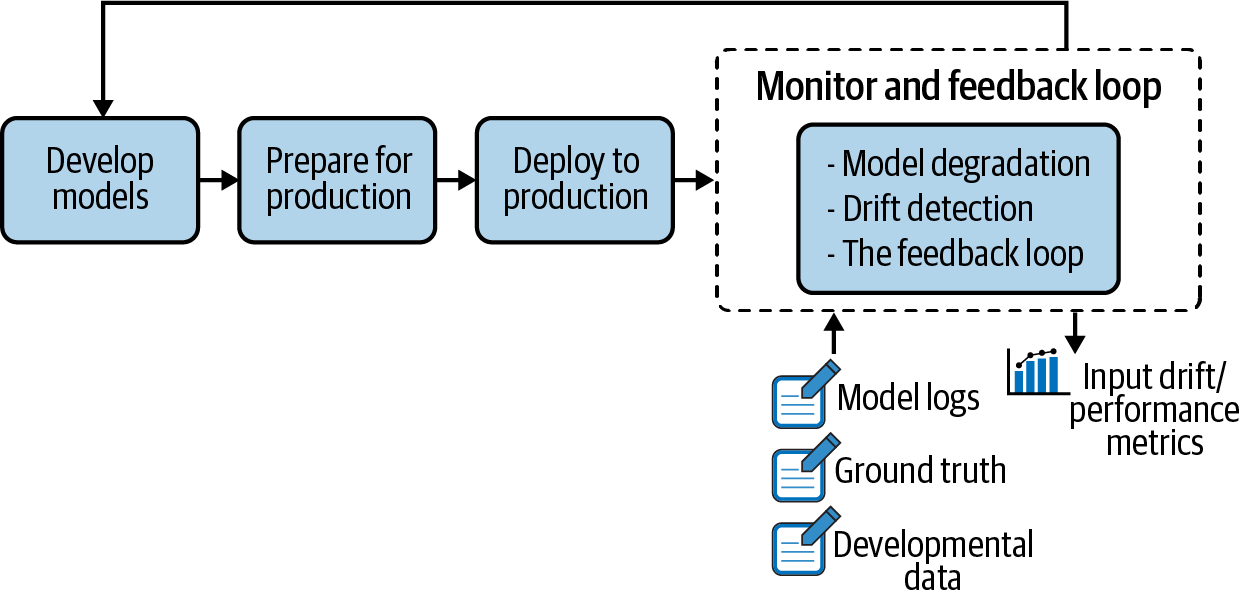
\includegraphics[width=.75\textwidth]{imlo_0701.png} \\

\vspace{\baselineskip}
\scriptsize \textbf{Source}: Treveil et al. (2020), Figure 7-1
\caption{Monitoring and Feedback in the MLOps Lifecycle}
\label{fig:monitoringfeedback}
\end{figure}

The feedback loop is important in that it triggers model retraining when required. The input drift and performance metrics are evaluated and assessed by the subject matter expert with reference to the relevant business key performance indicators. However, model retraining is not automatically triggered but depends on a number of considerations, for example:

\begin{itemize}
   \item \emph{Domain changes}: This indicates a shift or change in business requirements. For example, rather than extracting the maximum price for each item from a customer in a dynamic pricing model, the business is now also interested in maximizing the purchase of related products. Therefore, the existing prediction model may no longer be suitable o ruseful.
   \item \emph{Training cost}: Model training, especially for complex models or large training data sets, is time consuming and computationally costly. Organizations must consider these costs and the potential benefits or a more accurate prediction.
   \item \emph{Model performance}: Not every change in prediction accuracy or prediction error translates into a significant negative business impact. Some changes may be tolerable, in particular in light of the potential training time and costs for a new model version.
   \item \emph{Ground truth availability}: While continuous monitoring and logging can provide additional input data for training, it does not also provide the true target values. For example, while a dynamic pricing prediction service captures the input feature values, and whether a customer purchases a product offered at the predicted price, the true maximum price that a customer is willing to pay is not known.
\end{itemize}

Ground truth availability is a significant problem in many ML applications for at least the following three reasons:

\begin{itemize}
   \item \emph{Ground truth is not immediately or imminently available}. Consider the example of the dynamic pricing service that predicts the maximum amount a customer is willing to pay. The true maximum will never be known. Proxy variables can be used, for example whether a customer purchases a product at a given price, but these remain approximations. An example where ground truth is available late is loan application prediction, where the model predicts loan repayment or default of a customer. Loan repayment can only be fully captured at the conclusion of the loan duration, which may be months or even years after the prediction was made.
   \item \emph{Ground truth and prediction are decoupled}. Difficulties in capturing the ground truth can arise when different software applications are involved. For example, the dynamic pricing prediction model may not include a customer's identification as an input so that this information is not logged. This makes it difficult to later identify whether a purchase occurred for a particular price prediction.
   \item \emph{Ground truth not available for all classes}. Consider a fraud detection or prediction service. Predicted instances of fraud (''positive predictions'') may be investigated and be shown to be either true or false. that is, true and false positives will be known. However, not all negative predictions can or will be investigated because of their large number. Therefore, true negatives and false negatives will not be identified.
\end{itemize}

Input drift, that is, systematic changes to the frequency distributions of input values, may be caused by a non-stationary environment, for example, customers or markets changing over time, or by selection bias induced by the model itself. For example, a dynamic pricing application may drive away price conscious customers from the web store, changing the characteristics of the input values.

There are two main methods for input drift detection. The first method uses univariate statistical tests, for example, the  $\chi^2$ or Kolmogorov-Smirnov tests\footnote{\url{https://en.wikipedia.org/wiki/Chi-squared_test}} \footnote{\url{https://en.wikipedia.org/wiki/Kolmogorov-Smirnov_test}} to test whether two samples of input values are drawn from the same probability distribution. While these tests are simple and quickly carried out, they neglect the multi-variate distribution characteristics of the input data. 

The second approach is called the ''\emph{domain classifier approach}''. Conceptually, the old and new input values are considered as two classes (''domains''), and a classifier is trained on the input values themselves to predict whether an input observation belongs to the old class or the new class. If such a classifier can be trained to yield a classification accuracy better than chance, the old and new input data sets can be distinguished and must be considered different. 

The monitoring and feedback phase of the MLOps lifecycle requires software tools for logging of inputs, predictions, model explanations, and actions taken by the consumer of the prediction (e.g. the customer). This phase also requires access to model stores and online evaluation support. The latter tools allow for A/B testing or shadow testing, that is, to have two or more models in production and learn which one performs better based on live data. 

To illustrate basic logging in Python, the following code blocks extend the Flask microservice application introduced above\footnote{Complete file is available on \url{https://github.com/jevermann/busi4720-mlops/blob/main/flask_deploy_logging.py}.}. This example can illustrate only the most basic notions of logging events to a log file for later analysis. It uses the built-in, default \texttt{logging} package for Python.

The first code fragment sets up a logger to log the web requests to a file. A logger is characterized by its name and log level. Typical log levels, across many logging frameworks in most programming languages, are \texttt{DEBUG}, \texttt{INFO}, \texttt{WARN}, \texttt{ERROR} and \texttt{CRITICAL}, which are ordered in increasing order of severity. For example, \texttt{DEBUG} logging can be used to log a multitude of events that are useful to know about when creating a software application. However, DEBUG logging is generally not needed for applications in production. \texttt{INFO} logging captures events that are useful to determine the normal functioning of an application whereas \texttt{WARN} events in a log indicate conditions that are abnormal, but have not led to errors. Finally, \texttt{ERROR} events indicate errors in a software application but the application continues to work, while \texttt{CRITICAL} log events indicate errors that have led to the halting of a software application. The code below sets the logging level to \texttt{INFO} as routine events are to be captured. 

A file handler is added to the logger for writing the events to a file, rather than printing them on the console. As an alternative, a \texttt{RotatingFileHandler} may be used. This handler automatically limits the log file size and rotates logs when a file size exceeds the limit. In the example below, the 5 most recent logs are kept, while earlier log information is discarded. 

\begin{samepage}
\begin{pythoncode}
import logging.handlers

# Set up the logger:
req_logger=logging.getLogger(model_name+'.requests')
req_logger.setLevel(logging.INFO)
req_logger.addHandler(
    logging.FileHandler(
        model_name+'.requests.log'))
# req_logger.addHandler(
#     logging.handlers.RotatingFileHandler(
#         model_name+'.requests.log',
#         maxBytes=1000000,
#         backupCount=5))
\end{pythoncode}
\end{samepage}

With the request logger defined, the following code fragment shows how it can be used. The code block modified the \texttt{predict\_json()} and the \texttt{predict\_form()} functions to log the web request, together with the model name, the current time, and the remote internet address (the address of the web client or browser). Logging is done simply by calling the \texttt{info()} method of the request logger and providing the message to the be logged as well as the arguments to be inserted into that message. 

\begin{samepage}
\begin{pythoncode}
# Use the logger:
@app.route("/predict_json", methods=["POST"])
def predict_json():
    req_logger.info('%s TIME %s IP %s JSON %s', 
                    model_name, 
                    time.ctime(), 
                    request.remote_addr, 
                    request.json)
...
def predict_form():
    req_logger.info('%s TIME %s IP %s FORM %s',
                    model_name,
                    time.ctime(),
                    request.remote_addr,
                    request.form)
...
\end{pythoncode}
\end{samepage}

\begin{tcolorbox}[colback=code]
\subsubsection*{Hands-On Exercise}
\begin{enumerate}
\item Download the complete file from \href{https://github.com/jevermann/busi4720-mlops/blob/main/flask_deploy_logging.py}{GitHub}.
\item Define a second logger that writes to a different log file
\begin{itemize}
  \item You do not need to rotate this log file
  \item The definition of the second logger is analogous to that of the request logger
\end{itemize}
\item Add logging to the \texttt{predict\_json()} and the \texttt{predict\_form()} functions to capture the time, the three input values, and the prediction outcome in the log.
\begin{itemize}
   \item Replace the \texttt{\# TODO: Output logging goes here} comments with your code
   \item To make the log easy to analyze, write the information in CSV format. Make sure you quote the fields that need quoting.
\end{itemize}
\end{enumerate}
\end{tcolorbox}

\section{ML Governance}

In general, governance provides control, oversight, guidance, and makes strategically important decisions. ML governance in particular provides oversight, control, and directions to ML operations, and makes important strategic decisions around ML use in an organization. Governance often asks critical questions of management and operations to ensure that risks are appropriately managed and business value is realized or organizational goals are achieved. Figure~\ref{fig:mlgovernance} shows an 8-step process model for ML governance\footnote{The figure and the material in this section are adapted from Treveil et al. (2020).}.

\begin{figure}
\centering
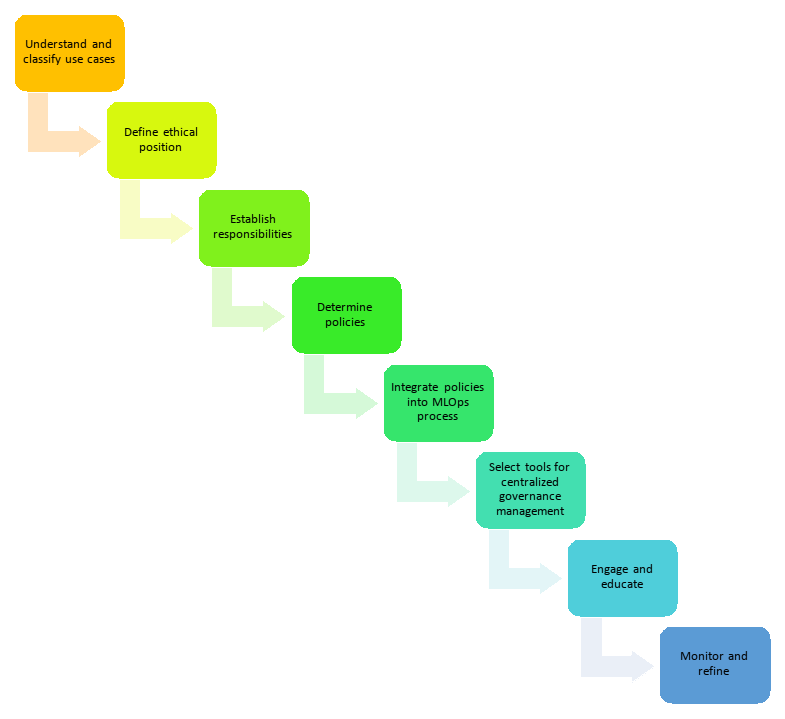
\includegraphics[height=3.25in]{governancegraphics.png}
\caption[ML Governance Phases]{ML Governance Phases (after Treveil et al. (2020), Chapter 8)}
\label{fig:mlgovernance}
\end{figure}

\begin{enumerate}
\item \emph{Understand ML Use Cases}. This step prompts the organization to understand the extent to which it uses ML models and for what purposes. Typical questions to ask (and to answer!) are the following:
\begin{itemize}
  \item Who are the consumers of the model outputs? Some models may be developed for internal consumption and decision making, while others may be customer facing.
  \item What regulations and legal constraints apply to each use case or model? Different industries and geographic or jurisdictional areas have different constraints. Organizations must identify the users of their models and the laws and regulations that apply. 
  \item What are the legal, financial, reputational risks of prediction errors? Answering this question ensures that effective model risk management is in place, as described above. 
  \item What is need for explainability or interpretability? Not all models need to be interpretable, and different models or model use cases may require different types of interpretability.
  \item What are the availability requirements for the various models? Not every model must provide 5-nines uptime, that is, be available 99.999\% of the time. Ensuring availability is generally costly. 
  \item What are the model lifetimes and likely rates of model deterioration? Knowing even approximate answers to this question can inform how fast or responsive the MLOps processes need to be. 
\end{itemize}

\item \emph{Define the Ethical Position}. This step guides how ML models will be used (or not used) by an organization. It examines the following questions:
\begin{itemize}
  \item How important are aspects like equality, privacy, human rights, democracy, bias? Answers to this question can, for example, inform the features that are used or excluded from prediction models, or what data is stored and logged from models in production. 
  \item How transparent should decision making be to the customers of the prediction models? Answers can inform the use of interpretable ML methods or the type of models deployed by the organization. 
  \item What level of responsibility for errors will or should the business assume? For some errors, the business or organization may accept financial responsibilities, for others it may try to deflect this responsibility by appropriate legal instruments (e.g. terms-of-service or licenses to use). 
  \item What is the potential for deception, manipulation, exploitation of model users? For example, a recommendation system that is used to increase sales may lead some users to purchase products or services they cannot afford, leading to financial hardship. As another example, consider recommendation systems for news articles that may lead users to biased or limited coverage. 
\end{itemize}

\begin{figure}
\centering
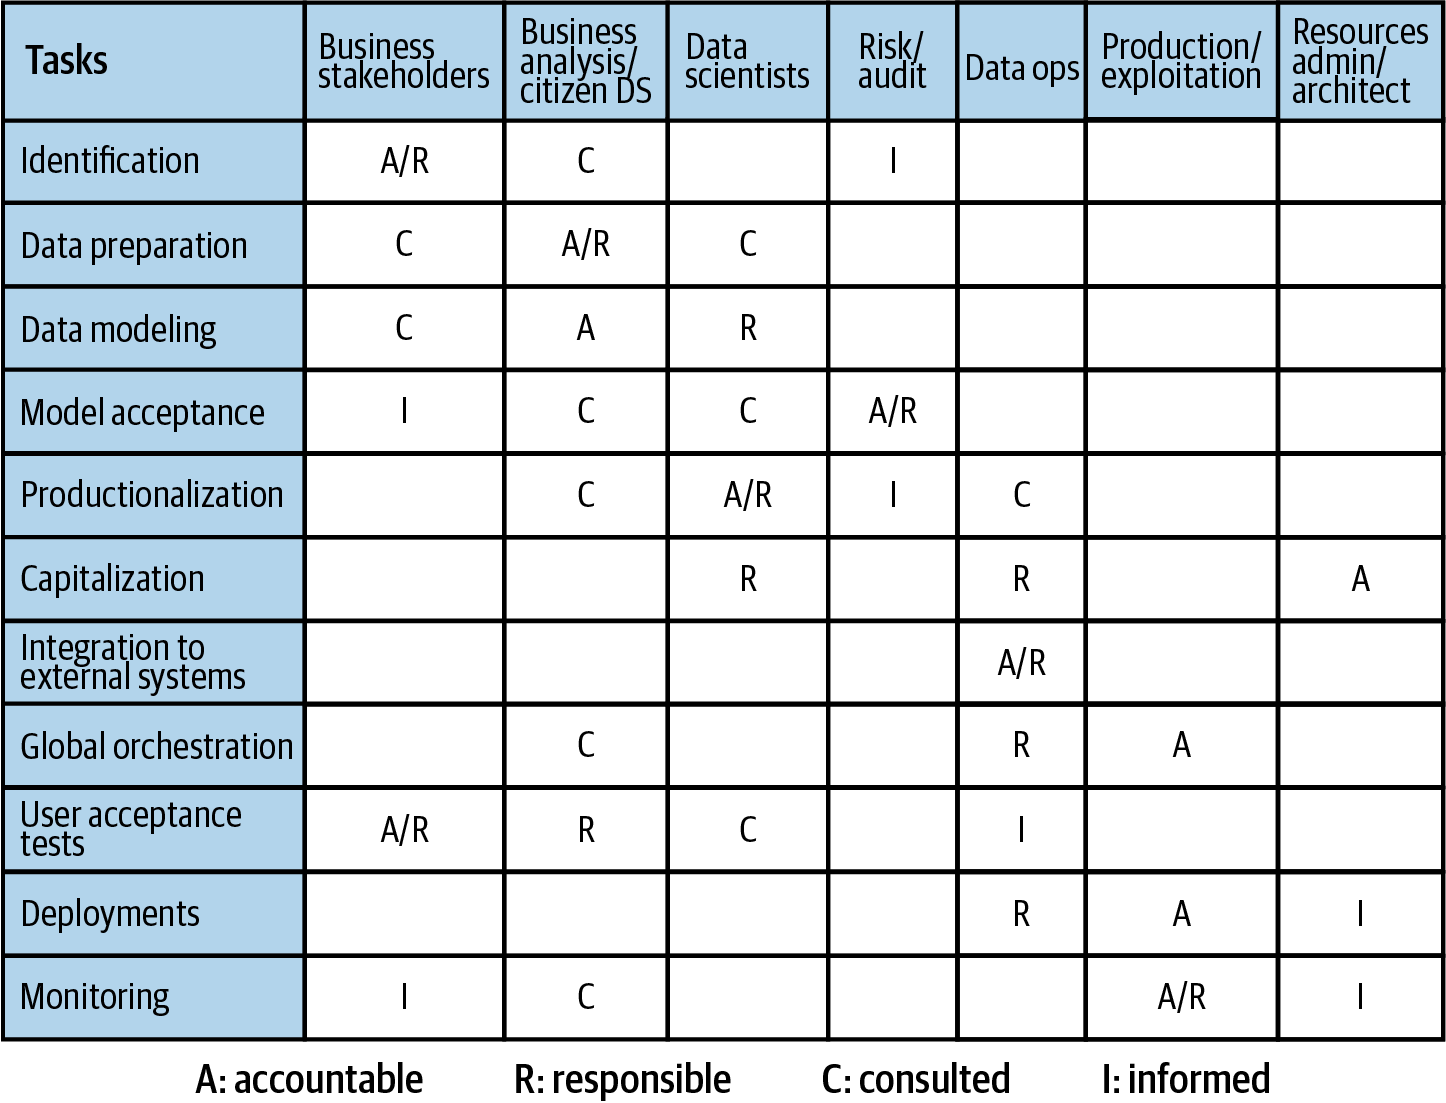
\includegraphics[width=.75\textwidth]{imlo_0806.png} \\

\scriptsize \textbf{Source:} Treveil et al. (2020), Figure 8-4
\caption{RACI Matrix for ML Governance}
\label{fig:mlraci}
\end{figure}

\item \emph{Establish Responsibilities}. This step essentially defines ''who will do what?''. A frequently used way to define responsibilities is through the use of a ''RACI'' matrix as in Figure~\ref{fig:mlraci}. RACI stands for ''responsible'', ''accountable'', ''consulted'', and ''informed''. This step of ML governance covers the following points:
\begin{itemize}
  \item Responsibilities must be defined at the strategic, tactical, and operational level. For example, who must be involved in model training (operational), who is allowed to sign-off on model risk (tactical) and who determines business goals or KPIs for a model (strategic)?
  \item Senior management sponsorship is important for the MLOps lifecycle. Without senior management recognizing the importance of ML models to the organization, and providing adequate resources and guidance for their development and use, ML and MLOps cannot function. 
  \item ML governance should be integrated into existing governance mechanisms. For example, organizations typically have IT governance mechanisms and a set of IT related policies and procedures. ML governance can extend these and define whether and how they apply to the MLOps lifecycle.
\end{itemize}

\item \emph{Define Policies}. This step answers the question ''how will we do that?''. Policies are formal and explicit rules that govern the details of what acceptable performance of the following issues means and how acceptable performance levels are achieved and documented. The following are the major MLOps aspects that require policies and some example questions to be answered by such policies:
\begin{itemize}
   \item Reproducibility and traceability: How is this achieved, measured, and verified? What are acceptable levels?
   \item Auditability and documentation: How much documentation and in what format is required? Where is the documentation maintained and who can access it?
   \item Sign-off between stages: Who has authority to, for example, select a model and move it to testing or deployment?
   \item Model verification: What verification tests must be performed? What are acceptable results? Who determines acceptable results? How are verification results documented? 
   \item Model explainability: What types of explainability are required for each model? Who is allowed to define such requirements? How can they be tested and documented?
   \item Model bias and bias testing: When and how must model bias be tested? What are acceptable levels of bias or fairness? Who determines them? How is bias testing documented?
   \item Model deployment mechanisms: Who has the authority to decide the choice of deployment mechanism and how are the resulting infrastructure requirements and model risk determined? How are decisions and their rationale to be documented? 
   \item Model monitoring: At what intervals is model performance monitored? Which metrics are recorded? How long are such records kept and maintained? Who has access to such records for analysis? What alarms are defined to identify model problems? Who must react how quickly to such alarms? 
   \item Data quality and data compliance: What are acceptable levels of data quality? How is it ensured, tested, and documented? Who is responsible for data compliance with legal and regulatory constraints? How is compliance demonstrated?
\end{itemize}
As noted, existing governance mechanisms, such as an IT use policy or an IT development or DevOps policy, should be applied when relevant. 

\item \emph{Integrate Policies into MLOps Process}. This step ensures that the relevant policies are actually applied and followed throughout the phases of the MLOps lifecycle. In particular, integration involves the following steps:
\begin{itemize}
   \item Formalize and automate MLOps processes: Automation of processes can ensure that the actions and decisions specified in policies are applied reliably and consistently. As far as possible, the activities required by a policy should be tool supported or automated. 
   \item Define controls: This step translates policy requirements into actionable or specific constraints and determines how control effectiveness can be measured. For example, if a policy specifies that a model must be globally explainable in terms of feature importance, an automated tool should prevent a model being deployed to production that does not have associated explanation test results in the model repository. A control for this may specify exactly what the model repository must contain. This also indicates how control effectiveness can be tested: All models in production should have the required explanation test results. 
   \item Define monitoring of controls: When and how frequently is control effectiveness monitored? Who performs such monitoring and who is responsible for actions in case of violations?
\end{itemize}

\item \emph{Implement Governance Tools}. As one of the core principles of MLOps is automation, it is unsurprising that ML governance mechanisms should also be automated and supported by appropriate software tools. This involves the following aspects:
\begin{itemize}
   \item Automate controls: As indicated above, controls should be automated in the software tools that form part of the MLOps tooling, such as model repositories, ML pipelines and ML workflow orchestration tools. 
   \item Logging of control violations: Once controls are defined, violations should be monitored and logged. This ensures accountability and auditability but is also useful for determining how MLOps processes or policies can be improved in the future. 
   \item Auditing of control effectiveness: Policy compliance and control effectiveness should be periodically audited by an independent auditor, that is, staff outside the MLOps process. Examples might be staff of the chief risk officer (CRO) or of the chief information officer (CIO) of the organization. 
   \item Policy and procedure maintenance: Policy repositories can support periodic policy and procedure evaluation, assessment and updates when required. They support policy dissemination and version management. 
\end{itemize}

\item \emph{Engage and Educate}. Policies and procedures are only effective if they are known and followed by those who they apply to. This step in the governance process includes the following aspects:
\begin{itemize}
   \item Communicate: Organizations have many different formal, semi-formal, and informal ways to communicate policies and procedures.
   \item Awareness: While communication makes policies and procedures available, awareness requires that MLOps participants consider the applicable policies throughout their daily work. 
   \item Training: Different training methods, online or in-person, individual or in groups, must be made available that cover both technical MLOps aspects as well as applicable policies, and how to best implement or comply with policies.
   \item Buy-in \& commitment: Successful MLOps and ML governance requires the buy-in and commitment to ML governance and efficient MLOps of all stakeholders and participants, at all levels of the organizations. 
   \item Culture: Successful MLOps is a cultural issue as much or even more so than a technical one. 
\end{itemize}

\item \emph{Monitor and Refine}. Just like deployed models must be continually monitored in the MLOps lifecycle, so must deployed policies and controls be continually monitored in ML governance. This includes:
\begin{itemize}
   \item Evaluating risk exposure: Governance, through the deployed policies, is designed to manage risk. An organization must periodically assess the actual risk exposure versus acceptable levels of risk and must, if necessary, adapt its governance mechanisms such as responsibilities, policies, or specific controls. 
   \item Evaluating policy adequacy: This examines whether policies are appropriate to control risk and ensure efficiency of the MLOps process.
   \item Evaluating control effectiveness: As noted above, control effectiveness must be continually monitored and evaluated. If necessary, controls must be strengthened. 
   \item Evaluating MLOps process performance: The overall efficiency and effectiveness of the MLOps process must be evaluated. This asks question such as: ''how long does it take to move a new model to production?'', ''how long does it take to recover from a production model problem?'', ''how often are there significant problems when moving a candidate model through testing?''. Recall that governance mechanisms are not only intended to manage risk but also to ensure efficiency. When process performance does not meet expectations, processes and policies may need to be adapted.
\end{itemize}
\end{enumerate}

\section{Review Questions}
\paragraph*{Introduction}
\begin{enumerate}[nosep]
    \item Why is the integration of a trained model into a production environment important, and what challenges can arise during this process?
    \item Provide an example of how a predictive model might be used in a business context and the potential risks involved.
    \item What are the three main purposes of MLOps?
    \item Why is the constant change in data a significant challenge for organizations using predictive models?
    \item Describe the composition of business analytics teams and the issues that may arise within such teams.
    \item What are the main principles around moving predictive analytics models into production according to MLOps?
    \item Define ''infrastructure as code'' and its importance in MLOps.
    \item Describe how MLOps intersects with machine learning, software engineering, and data engineering.
\end{enumerate}
\paragraph*{MLOps Lifecycle Overview}
\begin{enumerate}[nosep,resume*]
    \item Describe the two lifecycles that are combined in the MLOps lifecycle.
    \item How does the DevOps approach address the issues found in early software development practices?
    \item Explain the rationale behind combining the model development lifecycle and the DevOps lifecycle.
    \item How does the combined MLOps lifecycle address the integration of machine learning models into complex software applications?
    \item Using the example of a dynamic pricing web-store application, illustrate the steps involved in the MLOps lifecycle.
    \item Discuss the importance of formalized and automated processes in managing the MLOps lifecycle efficiently.
\end{enumerate}
\paragraph*{MLOps Roles and Requirements}
\begin{enumerate}[nosep,resume*]
    \item Describe the role of subject matter experts in the MLOps lifecycle. What are the requirements for subject matter experts to perform their role efficiently?
    \item Explain the responsibilities of data scientists in the MLOps process.
    \item How do data engineers support data scientists, and what are their main responsibilities?
    \item What automated tools do data scientists and data engineers require to perform their tasks efficiently?
    \item Discuss the role of data engineers in the MLOps lifecycle.
    \item Define the role of software engineers in integrating machine learning models. Describe the requirements of software engineers for effective collaboration and code management.
    \item What are the responsibilities of DevOps engineers in the MLOps lifecycle?
    \item Who are model risk managers and model auditors, and what are their primary responsibilities? What tools do model risk managers require?
    \item Describe the roles of ML engineers and ML architects in the MLOps lifecycle. Why is it important for ML engineers to quickly assess and adjust infrastructure capacities?
\end{enumerate}
\paragraph*{MLOps Tooling}
\begin{enumerate}[nosep,resume*]
    \item What are CI/CD tools, and how do they support the MLOps lifecycle?
    \item Define feature stores and their importance in managing data for ML models.
    \item Discuss the role of model registries in the MLOps lifecycle.
    \item What is the purpose of ML metadata stores, and how do they support MLOps?
    \item Explain the importance of model monitoring tools for deployed models.
\end{enumerate}
\paragraph*{MLOps Lifecycle Phases}
\begin{enumerate}[nosep,resume*]
    \item Describe the main phases of the simplified MLOps lifecycle.

    \item What are the main activities in and the outputs of the model development phase of the MLOps lifecycle?
    \item List some important questions related to data management that should be addressed during the model development phase.
    \item What are some key considerations for ensuring model fairness and mitigating bias during model development?

    \item What are the main tasks in and the inputs and outputs of the phase of preparing a model for production?
    \item What are the key considerations when selecting a runtime environment for a model?
    \item What are some key technical questions to consider when preparing a model for production?
    \item Describe the potential risks associated with deploying a machine learning model and how these risks can be assessed.
    \item List and explain some risk mitigation procedures that can be employed during the preparation for production phase.

    \item What are the main steps in and the inputs to deploying a model to production?
    \item Describe the components of a typical automated CI/CD pipeline for deploying machine learning models.
    \item What are the key considerations for ensuring scalability and reliability of model inference during deployment?
    \item Explain the importance of continuous monitoring in the deployment phase and what aspects should be monitored.
    \item Explain how a Flask microservice can be used to deploy a trained model.
    \item How can a neural network model be deployed in a browser-based web application using TensorFlowJS?

    \item Explain the concept of input drift and its potential impact on model performance.
    \item What are some aspects to consider when triggering model retraining?
    \item Discuss the challenges associated with ground truth availability and how they impact the monitoring and feedback phase.
    \item Describe two main methods for detecting input drift.
\end{enumerate}
\paragraph*{ML Governance}
\begin{enumerate}[nosep,resume*]
    \item What is the role of ML governance in the context of ML operations?

    \item Why is it important for an organization to understand its ML use cases?
    \item What are some critical questions to ask when understanding ML use cases?
    \item What are the potential consequences of not identifying the legal and regulatory constraints for ML models?

    \item Discuss some ethical considerations that organizations must address when using ML models.
    \item How can transparency in decision-making affect the deployment of ML models?
    \item Why is it important for an organization to consider the potential for deception or manipulation by ML models?

    \item Explain the concept of a RACI matrix and its role in ML governance.
    \item Why is senior management sponsorship important for the MLOps lifecycle?

    \item What are the key aspects of MLOps that require defined policies?
    \item Give examples of questions that need to be answered by policies related to model verification and monitoring.
    \item Provide examples of questions that policies should answer for reproducibility and traceability.

    \item Why is it important to formalize and automate MLOps processes?
    \item How can governance tools automate controls in the MLOps process?
    \item Explain the importance of logging control violations and auditing control effectiveness.

    \item List the aspects involved in engaging and educating MLOps participants.

    \item What is the importance of monitoring and refining policies and controls in ML governance?
    \item How can policy repositories support policy and procedure maintenance?
\end{enumerate}

